

\part{Training Coding Agents that Generalize across Tasks}
\label{part:generalizability}


\start{Overview of Part~\ref{part:generalizability}}
\autoref{part:scalability} presented two works for constructing scalable training data while preserving effectiveness. 
However, both works only focus on training and evaluation for a single task, whereas real-world coding agents are applied to a diverse set of applications.


In this part, we construct scalable training data for \emph{general-purpose coding agents} that generalize across a broad range of downstream tasks
This part contains two chapters.
In both chapters, we first conduct an in-depth analysis of the capabilities that the agent has not yet learned, but are required across diverse downstream tasks. 
Then we derive training data design principles based on the analysis results.

In \autoref{chap:hybrid-gym}, we investigate the transferable skills shared across diverse tasks by decomposing trajectories into fine-grained components (e.g., repository exploration) and derive a set of principles for training task design, such as matching the output format of downstream tasks and requiring non-trivial repository exploration.
Guided by these principles, we build our dataset on a set of scalable synthetic tasks, for instance, function localization and dependency search.
Experiments show that agents trained on our synthetic tasks effectively generalize to diverse real-world tasks (e.g., issue-solving, test generation, and library construction) that are not presented in the training data.

While \autoref{chap:hybrid-gym} presents principles for training task design, we observe that the concrete approach to accomplish the task is also crucial for training.
Particularly, experiments show that even successful trajectories generated from the same set of instances may have substantially different impacts in training.
In a \proposedWork (\autoref{chap:effective-analysis}), we propose a new work that aims to present principles for training trajectories.
We first conduct an analysis to investigate the characteristics that make a training trajectory beneficial or harmful in training from two aspects: the high-level problem-solving strategies and the concrete actions taken by the agent.
Then, we propose two trajectory augmentation methods to inject beneficial characteristics into the trajectories and remove harmful ones.













\chapter{Training General-Purpose Coding Agents with Scalable Tasks \textcolor{aquablue}{(\textit{completed})}}
\label{chap:hybrid-gym}



\begin{figure*}[t]
\centering
\resizebox{\linewidth}{!}{%
  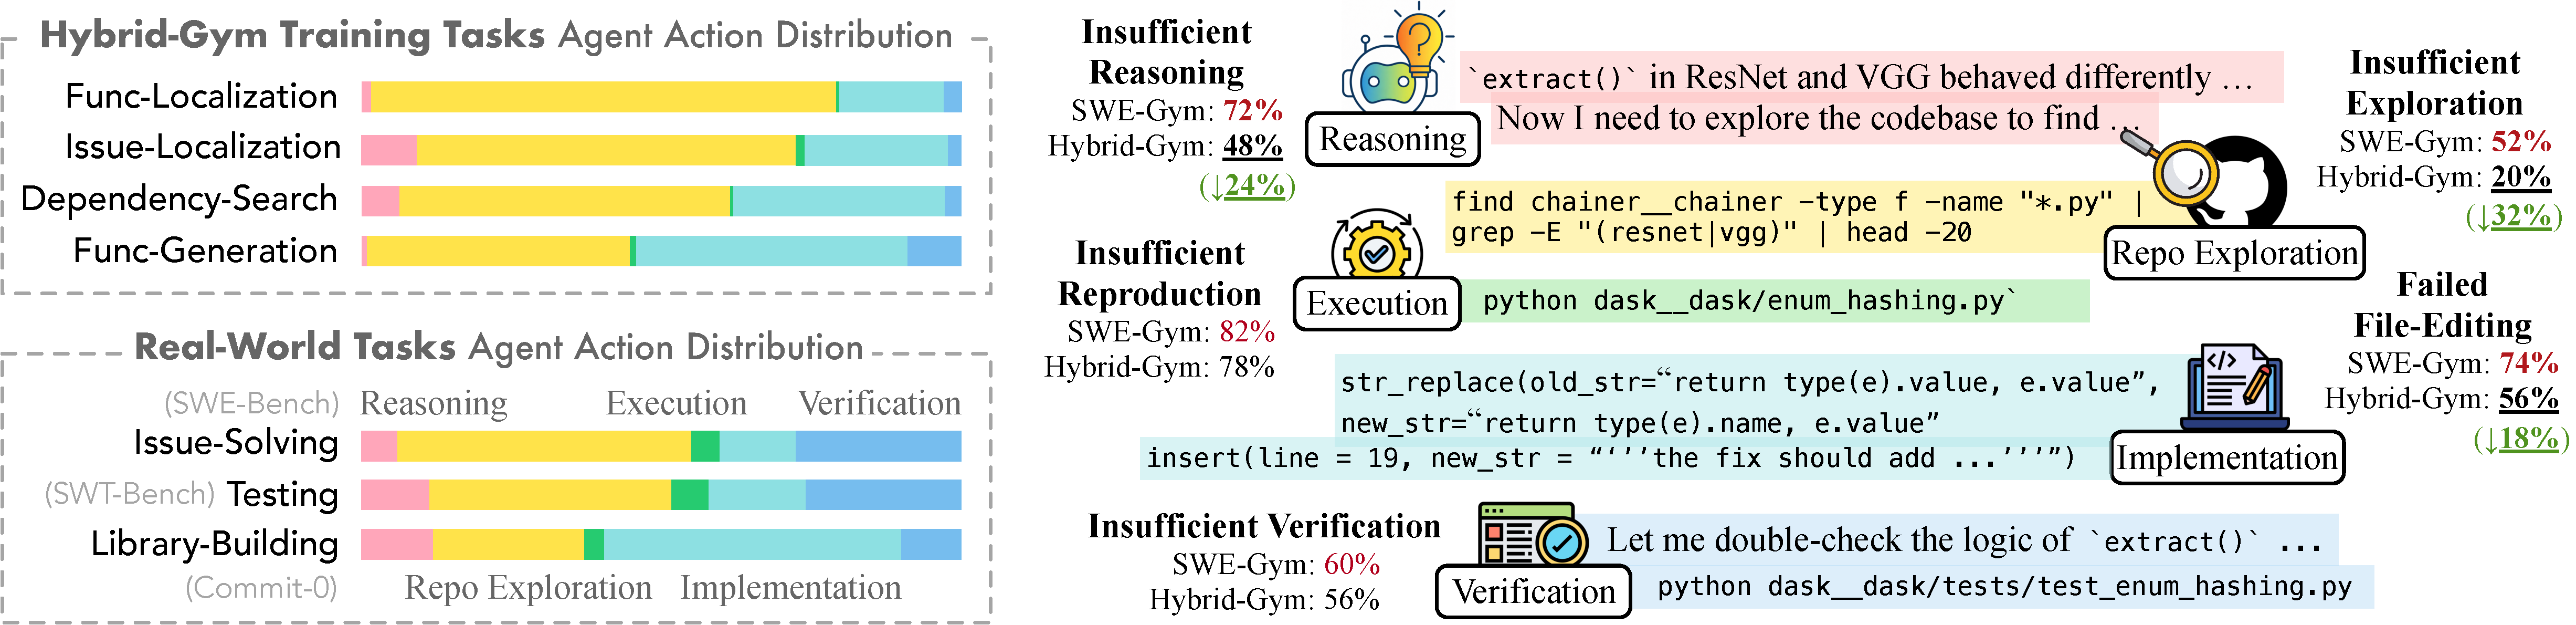
\includegraphics{HybridGym_figs/intro.pdf}%
}
\caption{(\textit{\textbf{Left}}) We decompose general coding agent tasks into a set of intermediate components and compute the percentage of agent actions spent on each component. Our training tasks partially cover verification and fully cover reasoning, repository exploration, and implementation, which consist of around 68\% of the actions.
\textit{(\textbf{Right})} Example actions for each component. Compared to a baseline training method, SWE-Gym~\cite{swegym}, training with our \repostmethodname significantly reduces failures due to insufficient reasoning, insufficient exploration, and failed file editing, improving the final resolved rate on SWE-Bench Verified from 10.6\% to 15.0\%. 
}
\label{fig:intro}
\end{figure*}

\section{Introduction}

% [Para-1: an overview of coding agent and its training]
Recent advances in large language models have enabled LM-based agents~\citep{sweagent,openhands} to tackle real-world coding tasks, with rapid progress in benchmarks such as the SWE-Bench issue resolution benchmark~\citep{swebench}.
While most existing methods only focus on the issue-solving task~\citep{swegym,R2EGym,swe-smith}, the application of coding agents can be diverse in real-world usage. A recent study show that more than 70\% of the real-world prompts target other software engineering tasks~\citep{valerie-interaction}.

% [Para-2: motivate task transfer]
As shown in a concurrent work~\citep{swe-play}, training on a single task can lead to overfitting and is not sufficient for generalizing to general coding agent tasks.
In particular, agents trained on issue solving do not transfer reliably to tasks such as test generation or library implementation. This calls for training coding agents with stronger \textbf{task generalization} capabilities.
Yet, in the current literature, task transferability for coding agents remains underexplored. 
In this work, we ask: what commonalities do real-world coding tasks share? How can we design training tasks that transfer effectively across a broad range of coding agent tasks?

% [Para-4: our analysis results]
To answer these questions, we start by decomposing real-world tasks into intermediate components (e.g., reasoning and repo-exploration) and analyzing the model's capabilities on each.
These results are shown in \autoref{fig:intro}.
We observe that a large number of actions in successful trajectories are spent on reasoning, repo-exploration, and implementation.
These categories also remain challenging for current coding agents.
For instance, even after finetuning on issue-solving~\cite{swegym}, the agent still has file editing failures for the majority of the examples.

Fortunately, these intermediate components can be isolated from the construction of coding environments with executable repositories (e.g., with all Python packages required by the repository installed).
In previous work, setting up executable repositories is often viewed as a prerequisite for constructing training examples. This typically involves a series of complex steps such as package installation and test generation, which is still challenging for agents~\cite{swe-play} and time-consuming for human~\cite{swegym,swe-smith,R2EGym}.
Based on the observation from our analysis, we ask: \textbf{can we design a set of tasks that cover the major components for coding practice: reasoning, repo-exploration, and implementation, but do not require executable repository setup?}


% [parap-5: in this paper]
In this paper, we present \repostmethodname, a large-scale coding agent training dataset containing a suite of coding agent training tasks that only require simple environment setup.
Based on our analysis summarized in \autoref{fig:intro}, we present a list of principles for training task design: the task needs to 
(1) match the output format of downstream tasks;
(2) include a repository exploration process; and 
(3) require non-trivial reasoning.
For scalability concerns, we further require that the task (4) must \emph{not} require a complicated environment setup.
Example tasks include function localization, issue localization, dependency search, and function generation.
As shown in \autoref{fig:intro}, even without setting up executable repositories, all our tasks cover the major intermediate components of multiple downstream tasks, and such components are achieved with a similar set of actions across tasks. 
After training on \repostmethodname, the agent has significantly lower failure rates in reasoning, exploration, and file-editing compared to the baseline training method~\cite{swegym}.


% [para-6: experimental results]
We conduct experiments on three real-world coding agent tasks: SWE-Bench issue-solving~\citep{swebench}, SWT-Bench test generation~\citep{swt-bench}, and Commit-0 library generation~\citep{commit0}.
Without training on any of the downstream tasks, \repostmethodname demonstrates strong task transferability on all three tasks, improving Qwen2.5Coder-32B by 25.4\% / 7.9\% / 5.1\% on SWE-Bench Verified / SWT-Bench Verified / Commit-0 Lite, which achieves comparable performance to in-domain datasets (i.e., data built for the downstream tasks). 
Additionally, we also improve the performance of training on existing in-domain datasets by combining with \repostmethodname (e.g., we improve SWE-Play~\citep{swe-play} by 2.4\% / 4.9\% on SWE-Bench Verified / SWT-Bench Verified).


% [para-7: controlled experiment results]
To provide insights to future research on coding agent training, we conduct a series of controlled experiments to reveal what transfers and what does not for coding agents.
In addition to validating our task design principles that require output format matching, repo-exploration, and non-trivial reasoning, we observe that even successful trajectories of the same set of instances can lead to markedly different impact.
Repository diversity improves training effectiveness, but training on the same repositories used in evaluation does not inflate performance gains.
The results emphasize the importance of teacher model selection and data selection.





\begin{table}[t]
\centering
\resizebox{\linewidth}{!}{%
\begin{tabular}{llcccc@{\hspace{4pt}\vrule width 0.6pt\hspace{4pt}}ccc}
\toprule
\bf Command & \bf Example & \bf Func-Localize & \bf Issue-Localize & \bf Dep-Search & \bf Func-Gen & \bf SWE-Bench & \bf SWT-Bench & \bf Commit-0 \\
\midrule
grep & \texttt{grep -i "pipeline"} & 31.3\% & 36.1\% & 48.4\% & 89.9\% & 35.4\% & 37.4\% & 5.3\% \\
find & \texttt{find . -type f -name "least\_angle.py"}           & 17.5\% & 11.1\% & 21.4\% & 8.7\%  & 16.2\% & 21.5\% & 31.6\% \\
cd   & \texttt{cd /workspace/scikit-learn}                       & 21.9\% & 31.5\% & 2.0\%  & 0.0\%  & 26.7\% & 0.0\% & 5.3\% \\
ls   & \texttt{ls -la}                                           & 6.6\%  & 2.3\%  & 3.7\%  & 0.0\%  & 2.4\%  & 12.4\% & 36.8\% \\

\bottomrule
\end{tabular}%
}
\caption{The use of Linux commands for repository exploration in our proposed training tasks (left) and downstream tasks (right). We show the percentage of each command used in the agent steps targeting repository exploration.
}
\label{tab:cmd-category}
\end{table}


\begin{table}[t]
\centering
\resizebox{\textwidth}{!}{%
\begin{tabular}{lcccc@{\hspace{4pt}\vrule width 0.6pt\hspace{4pt}}ccc}
\toprule
\bf Category & \bf Func-Localize & \bf Issue-Localize & \bf Dep-Search & \bf Func-Gen & \bf SWE-Bench & \bf SWT-Bench & \bf Commit-0 \\
\midrule
Analysis and reasoning        & 1.6\%  & 9.3\%  & 6.3\%  & 0.9\%  & 6.0\%  & 11.4\% & 1.3\% \\
Repository exploration        & 77.9\% & 66.2\% & 55.5\% & 44.6\% & 49.1\% & 40.3\% & 27.3\% \\
Execution of existing code    & 0.1\%  & 0.3\%  & 0.1\%  & 0.2\%  & 4.7\%  & 6.3\%  & 3.7\% \\
Solution implementation       & 17.4\% & 23.9\% & 35.3\% & 45.3\% & 12.7\% & 16.2\% & 53.8\% \\
Solution verification         & 3.0\%  & 0.3\%  & 2.8\%  & 9.0\%  & 27.6\% & 25.9\% & 10.9\% \\
\bottomrule
\end{tabular}%

}
\caption{We categorize the agent's actions based on the intermediate components of the task, where the categories are pre-defined. 
}
\label{tab:action-category}
\end{table}

\begin{figure}[t]
\centering
\resizebox{\linewidth}{!}{%
  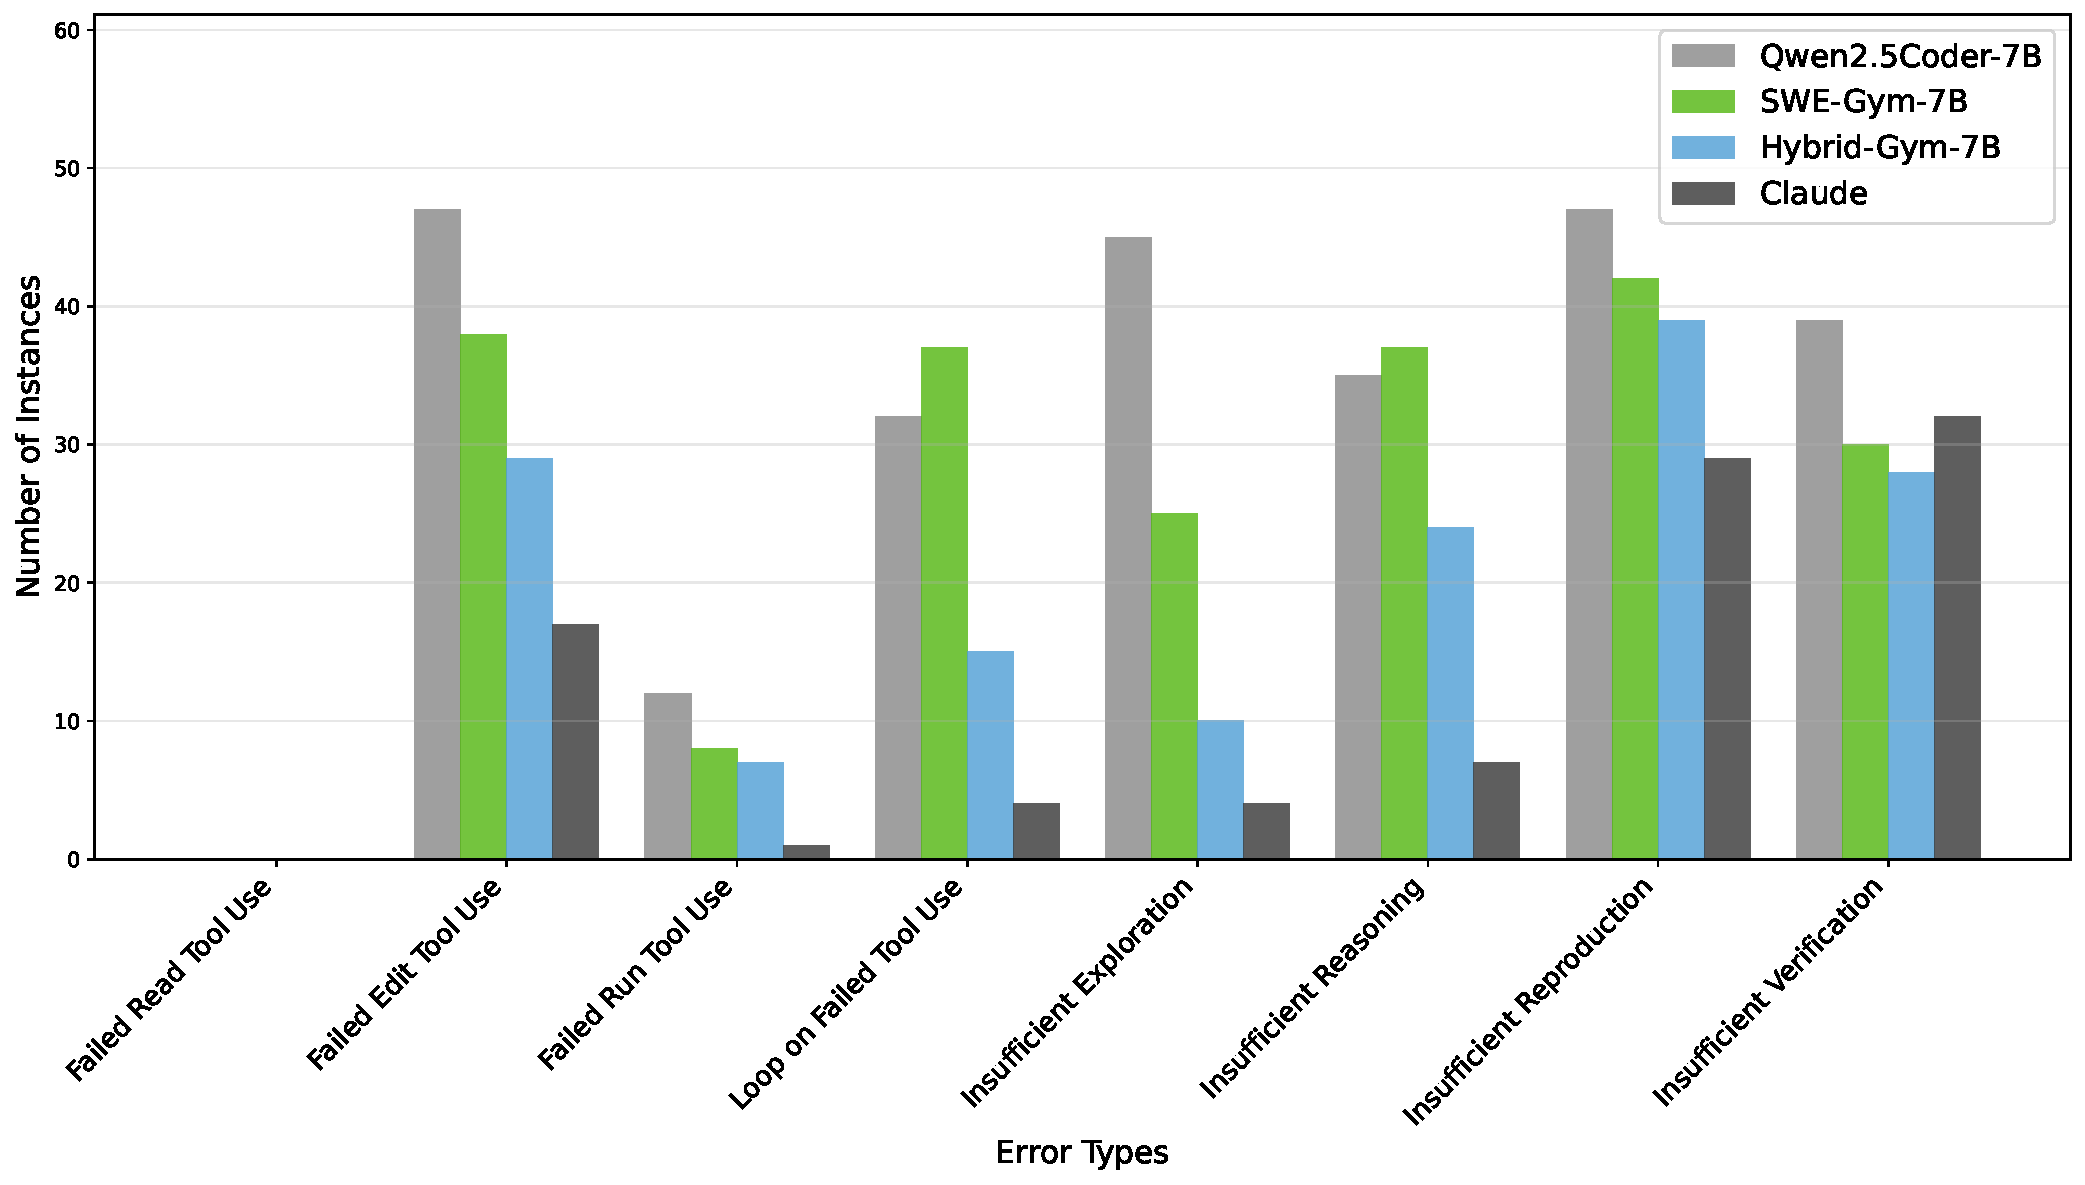
\includegraphics{HybridGym_figs/error_analysis.pdf}%
}
\caption{The error analysis of different methods on 50 instances sampled from SWE-Bench Verified.}
\label{fig:error-analysis}
\end{figure}








\section{Methodology}
\label{sec:methodology}
In this section, we first guide training task design by analyzing the commonalities shared among coding tasks and agent capabilities (\S\ref{sec:analysis-methodology}).
Based on the analysis results, we introduce a list of task design principles (\S\ref{sec:principle}) and present the four \repostmethodname tasks that satisfy all the principles (\S\ref{sec:tasks}).
Finally, we conduct a comparison between our training tasks and real-world coding tasks (\S\ref{sec:task-verification}).

\subsection{Analysis of Coding Agent Task Transferability}
\label{sec:analysis-methodology}
With the ultimate goal of designing training tasks that transfer to diverse downstream tasks, we first investigate the commonalities shared by real-world tasks by answering:
[\textbf{RQ1}] What are the commonalities of the components (i.e., high-level problem-solving steps) to complete real-world coding tasks?
[\textbf{RQ2}] What are the commonalities of the concrete actions (i.e., commands) taken by the agents?
Since effective training must target capabilities the agent has not yet learned, we also ask
[\textbf{RQ3}] What are the abilities that the agent has not learned but are required for task completion?

\start{Analysis Setup}
Following prior works~\citep{swegym,R2EGym,swe-play}, we adopt the rejection sampling finetuning setting, where we finetune Qwen2.5-Coder-7B/32B on the successful trajectories generated for the training tasks. 
We conduct the analysis based on 200 successful trajectories sampled from each task, which are generated by Claude-4.5~\cite{claude45} using OpenHands CodeAct as the agent scaffold~\cite{openhands}


\start{Task Analysis: Decomposition of Coding Tasks}
To answer \textbf{RQ1}, we first decompose general coding agent tasks into five intermediate components: reasoning, repo-exploration, execution of existing code, solution implementation, and verification. 
We then use o3-mini~\cite{o3_mini} to categorize each agent action by the component it targets.
We manually examined 20 cases and made the same categorization as o3-mini in all the cases.

Results in \autoref{tab:action-category} show that (1) The action distribution across different components is similar for the three downstream tasks, with repo-exploration accounting for the largest share.
(2) We notice that around 70\% of the actions fall into categories that do not require setting up executable repositories: reasoning, repo-exploration, and implementation.
This is notable because executable repository setup is complicated and challenging for both humans and agents~\cite{swe-smith,swe-play} and is the bottleneck of constructing scalable training datasets.
Our analysis hence suggests a key direction: training tasks that avoid executable repository setup can also be beneficial.


\start{Task Analysis: Concrete Actions Used in Coding Tasks}
To answer \textbf{RQ2}, we analyze the concrete agent tools used in each task. 
The tools built for the OpenHands agent~\cite{openhands} include bash command execution (\texttt{execute-bash}), file viewing (\texttt{view}), and file editing (\texttt{str-replace}).
Results in \autoref{tab:action-category} show that all three tools are heavily used across downstream tasks. This suggests that \emph{the agents need to learn all the tools in training.}

For the bash execution tool, we further analyze the specific commands issued by the agent. \autoref{tab:cmd-category} shows that different tasks rely on highly similar repo-exploration commands, such as grep, find, cd, and ls, suggesting that \emph{repo-exploration skills could be broadly transferable across tasks.}


\start{Agent Capability Analysis}
To answer \textbf{RQ3}, under the setting of distillation-based training, we conduct an error analysis for the untrained student model (Qwen2.5Coder-7B, \citet{qwen25coder}), the student model trained on a baseline dataset (SWE-Gym, \citet{swegym}), and the teacher model (Claude-4.5, \citet{claude45}).
We define error categories along two axes: (1) failures in the intermediate components identified in our previous analysis, and (2) failures in the use of each tool.
We then prompt an LLM to label whether each agent trajectory exhibits these failures.


\autoref{fig:error-analysis} presents the error analysis results.
We observe several error categories where the fine-tuned model’s failure rate remains far higher than the teacher model’s: insufficient repo-exploration, insufficient reasoning, and failure/loop on the file-editing tool.
This suggests that \emph{these capabilities still have substantial room for improvement.}





\subsection{Principles for Training Task Design}
\label{sec:principle}
We summarize the analysis results in \S\ref{sec:analysis-methodology} as follows:
(1) reasoning, repo-exploration, and implementation are the dominant intermediate components shared across coding-agent tasks;
(2) The concrete types of commands to complete these components are also similar across tasks; and
(3) The performance gaps between the student and teacher models are still large for the above categories and file editing.

Based on the task commonalities and the agents' capabilities, we present the following principles for training task design:

\quad [\textbf{Principle 1}] The tasks should have the same output format as the downstream tasks.
For the downstream tasks in our evaluation, the format is generating a code patch in the codebase, which requires file editing.
A counterexample for training tasks is a variant of our issue-localization task, where we only need the agent to generate the plan to resolve the issue in the message, without making any code changes.

\quad [\textbf{Principle 2}] The tasks should involve a meaningful repository-exploration phase. 
A counterexample is a script-level code generation task (e.g., HumanEval~\cite{codex}). 
Although we can still provide a repository as context by putting the solution template file inside an empty repository, it does not involve any file localization.

\quad [\textbf{Principle 3}] The tasks should require a non-trivial level of reasoning to complete. Namely, the agent must make substantive decisions, such as choosing the problem-solving strategy, generating the precise tool call arguments, and writing the code.
A counterexample is a simple string-replacement task where we provide the exact edit location and the old/new strings. The agent can succeed by a single \texttt{str-replace} call without inspecting the codebase.


With the observation that all the major components: reasoning, exploration, and implementation, do not require an executable repository, we further require the training tasks to be scalable (i.e., easy to generate new instances):

\quad [\textbf{Principle 4}] The task setup should not require substantial effort. For instance, the task should avoid installing packages for the entire repository or generating executable test files, which are challenging for both humans and agents.

In \S\ref{sec:exp}, we will show that all \repostmethodname tasks satisfy all four principles and generalize well to multiple downstream tasks.
In contrast, \S\ref{sec:controlled-exp} will show that all three counterexample tasks mentioned above do not yield effective task transfer.


\begin{table}[t]
\centering
\resizebox{0.5\linewidth}{!}{%
\begin{tabular}{lccc}
\toprule
\bf Dataset & \texttt{execute-bash} & \texttt{view} & \texttt{str-replace} \\
\midrule
Func-Localize  & 5.55  & 4.43 & 1.16 \\
Issue-Localize & 9.37  & 7.76 & 5.15 \\
Dep-Search     & 1.78  & 3.12 & 1.89 \\
Func-Gen       & 0.53  & 1.75 & 1.47 \\
\midrule
SWE-Bench      & 10.65 & 6.88 & 3.65 \\
SWT-Bench      & 16.54 & 6.09 & 5.16 \\
Commit-0       & 18.40 & 21.20 & 36.40 \\
\bottomrule
\end{tabular}%
}
\caption{The average number of OpenHands tools called in each trajectory.}
\label{tab:openhands-tool-distribution}
\end{table}

\begin{table}[t]
\centering
\resizebox{\linewidth}{!}{%
\begin{tabular}{lcccccccc}
\toprule
\multirow{2}{*}{\bf Model} &
\multicolumn{2}{c}{\bf Func-Localize} &
\multicolumn{2}{c}{\bf Issue-Localize} &
\multicolumn{2}{c}{\bf Dep-Search} &
\multicolumn{2}{c}{\bf Func-Gen} \\
\cmidrule(lr){2-3}\cmidrule(lr){4-5}\cmidrule(lr){6-7}\cmidrule(lr){8-9}
& Success \% & Non-Empty \% & Success \% & Non-Empty \% & Success \% & Non-Empty \% & Success \% & Non-Empty \% \\
\midrule
Qwen2.5Coder-7B   & 0.0\%  & 50.0\% & 3.3\%  & 16.7\% & 6.7\%  & 60.0\%  & 5.0\%  & 70.0\% \\
Qwen2.5Coder-32B  & 40.0\% & 95.0\% & 33.3\% & 83.3\% & 56.7\% & 86.7\%  & 25.0\% & 95.0\% \\
\midrule
Claude-4.5        & 70.0\% & 100.0\% & 63.3\% & 100.0\% & 80.0\% & 100.0\% & 50.0\% & 100.0\% \\
\bottomrule
\end{tabular}%
}
\caption{Performance of the student and teacher models on a subset of instances sampled from each training task.}
\label{tab:distillation-sanity-check}
\end{table}


\subsection{\repostmethodname Tasks}
\label{sec:tasks}

In this section, we introduce four \repostmethodname tasks that satisfy all the principles above.
% We provide the prompt for each task in Appendix \ref{app:data-construction}.

\start{Function Localization}
To boost repository exploration (principle 2), we design a task to localize a function in the entire codebase:
given a short description, the agent needs to identify the corresponding function in the codebase.
To satisfy Principle 1, which requires generating a code patch as the outcome, we require the agent to write a docstring containing the fix plan. 
We evaluate the task by checking whether a docstring is added for the correct function.
This task requires substantial reasoning (principle 3), as the agent needs to understand the code content and conduct an effective and targeted search over the entire repository, which contains 2,925 functions on average in our training set.

\start{Issue Localization}
Function localization aims to locate the code based on the description, and issue localization locates the problematic code based on an issue.
Given a GitHub issue, the task is to locate the relevant code in the repository and leave a comment containing a plan to fix the issue.
We evaluate the task by checking whether a comment is generated in the same file where the actual fix is located. 

Compared to the issue-solving task used in most prior work, constructing issue localization data does not need test execution for evaluation and can be instantiated from arbitrary GitHub issues.
However, it still requires reasoning effort on analyzing the issue, exploring the repository, planning the fix, and making successful file-editing actions.

\start{Dependency Search}
We have the third task that targets code localization, which requires file-editing, repo-exploration, and reasoning: given a function, the agent must identify all functions or classes it directly calls.
Similar to the above two tasks, we require adding comments to all these dependent modules.
To obtain the ground truth, we adopt \texttt{Jedi}, a static Python analysis tool, to resolve imported names to their defining modules.
Solving this task requires the agent to locate the target function, extract the referenced names, resolve each name to the correct module, and successfully edit the relevant files.
This is non-trivial because a codebase may contain multiple modules with the same name, and only one corresponds to the actual call.

\start{Function Generation}
Beyond the localization tasks that only aim to generate comments, we design the function generation task that requires actual code generation. 
Given a function in a codebase, we use an LLM to generate a description of its functionality.
Then we remove the function body and ask the agent to re-implement it.
To evaluate the implementation with test cases while avoiding repository installation, we adapt the RepoST~\cite{repost} method to the coding agent setting, which extracts the target function and its dependencies to a separate script and generates tests.

Here we highlight that generating \emph{executable test scripts} is substantially easier and more cost-efficient than setting up \emph{executable repositories}.
To execute the test script, we only need to install the packages needed by the extracted function and its dependencies (2.1 packages on average), while installing the entire repository requires 26.5 packages on average.
Furthermore, compared to \emph{generating a new test file} that requires understanding the repository structure and resolving relative imports, it is substantially easier to \emph{produce tests for a separate script}, which only requires seq-to-seq generation, without any agentic frameworks, making the setup process cost-efficient.

We emphasize that \repostmethodname is not limited to the specific tasks introduced here: other task designs may also satisfy our principles.
It is also possible to construct variants of our tasks, such as localizing multiple functions, or finding the empty function before generating the function body. We leave the exploration to future works. 

\begin{table}[t]
    \centering
  \resizebox{0.7\linewidth}{!}{%
    \begin{tabular}{lccccc}
      \toprule
      \bf Dataset & \bf \# Trajs & \bf \# Repos & \bf Avg Steps & \bf \# Images & \bf Cost \\
      \midrule
      SWE-Gym   & 491   & 11  & 40.2 & 2.4k & unknown \\
      R2E-Gym   & 3,321 & 10  & 33.2 & 4.5k & unknown \\
      SWE-Smith & 5,016 & 128 & 26.7 & 128  & 2.32\textcent \\
      SWE-Play  & 704   & 28  & 72.9 & 28   & unknown \\
      \midrule
      \repostmethodname & 4,470 & 762 & 39.1 & 2 & 0.07\textcent \\
      \hdashline
      \quad Func-Localize  & 1,438 & 226 & 29.0 & 1 & 0.02\textcent \\
      \quad Issue-Localize & 1,978 & 263 & 52.4 & 1 & 0.00\textcent \\
      \quad Dep-Search     & 502   & 120 & 26.9 & 1 & 0.00\textcent \\
      \quad Func-Gen       & 552 & 306 & 28.6 & 1 & 0.56\textcent \\
      \bottomrule
    \end{tabular}%
  }
  \caption{Statistics of \repostmethodname and its subsets.
  Following SWE-Smith, we report the average per-instance cost of setting up the training environment for rollout.
  Compared to existing datasets, \repostmethodname covers more repositories and requires only 2 docker images to build all training instances.}
  \label{tab:stat}
\end{table}

\begin{figure}[t]
    \centering
    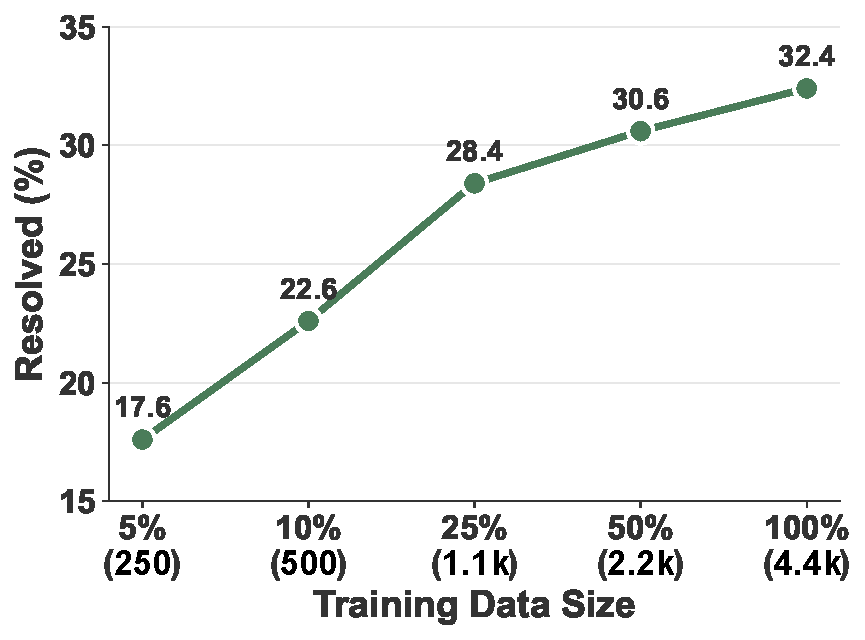
\includegraphics[width=0.6\linewidth]{HybridGym_figs/fig_scaling_law_v2.pdf}
  \caption{Scaling law analysis. Performance on SWE-bench Verified improves consistently as training data size increases from around 5\% (250 trajectories) to 100\% (4.4k trajectories).}
  \label{fig:scaling}
\end{figure}



\subsection{Verification of \repostmethodname Tasks}
\label{sec:task-verification}
In this section, we verify that our training tasks share commonalities with real-world tasks and remain challenging for the student models we use: Qwen2.5Coder 7B and 32B.

\start{\repostmethodname tasks cover the majority of intermediate components in multiple real-world tasks}
As shown in \autoref{tab:action-category}, all the training tasks cover reasoning, repo-exploration, and implementation, and the function-generation task additionally includes solution verification.
We note that although our training tasks do not explicitly include executing existing code, it typically accounts for only a small fraction of an agent's trajectory.

\start{\repostmethodname trajectories contain similar actions with real-world tasks}
As shown in \autoref{tab:cmd-category}, the training tasks use a similar set of bash commands for repo-exploration as the real-world coding tasks.
Similarly, \autoref{tab:openhands-tool-distribution} shows that the training tasks cover the full set of OpenHands tools used in downstream tasks.
Together, these results suggest that both the high-level problem-solving components and the concrete actions that achieve them can transfer across \repostmethodname tasks and downstream tasks.


\start{\repostmethodname tasks are still challenging for models without finetuning}
Under the setting of distillation learning, a training task is useful only if there is a performance gap between the student and teacher models
As a sanity check, before generating training data, we sample 20-30 instances from each task and evaluate the teacher model (claude-4.5-Sonnet) and student models (Qwen2.5Coder, 7B and 32B).

\autoref{tab:distillation-sanity-check} show that Claude-4.5 achieves substantially higher success rates than Qwen2.5Coder-32B on all four tasks, with gaps ranging from 23.3\% to 30.0\%. This confirms that all tasks provide sufficient room for effective distillation.







\section{Results}
\label{sec:exp}

\subsection{Experimental Setup}
\start{Statistics of \repostmethodname}
\autoref{tab:stat} presents the statistics of \repostmethodname and existing datasets. 
Based on the scalable training tasks, we collect 4.4k trajectories from 762 repositories using only two Docker images.
The environment construction cost is only 0.07\textcent per example, which is 16× lower than SWE-Smith~\cite{swe-smith}.
Trajectory lengths vary by task, ranging from 26.9 to 52.4 agent steps, which are comparable to the issue-solving trajectories in prior datasets, suggesting that our tasks retain a meaningful level of complexity.
The trajectories are obtained from the combination of Claude-4.5~\cite{claude45}, Claude-3.7~\cite{claude37}, and Qwen3-235b~\cite{qwen3}.
% We provide dataset details in Appendix~\ref{app:data-construction}.


\begin{table*}[t]
\centering

\resizebox{\textwidth}{!}{%
\begin{tabular}{c@{\hspace{2pt}}c@{\hspace{2pt}}c@{\hspace{2pt}}c l ccc cc c}
\toprule
\multicolumn{4}{c}{ \multirow{2}{*}{\bf Training Tasks} } &
\multirow{2}{*}{\bf Training Dataset} 
& \multicolumn{3}{c}{Issue Solving (swe)} 
& \multicolumn{2}{c}{Test Generation (swt)} 
& \multicolumn{1}{c}{Library Build (cmt)}\\
& & & &
& \multicolumn{3}{c}{\bf SWE-bench Verified} 
& \multicolumn{2}{c}{\bf SWT-Bench Lite \& Verified} 
& \multicolumn{1}{c}{\bf Commit-0 Lite} \\
\cmidrule(lr){1-4}
\cmidrule(lr){6-8}\cmidrule(lr){9-10}\cmidrule(lr){11-11}
swe & swt & cmt & syn
& & Resolved \% & Localized \% & Non-Loop \%
& Lite Resolved & Verified Resolved
& Resolved \% \\
\midrule

\sdlrow & \multicolumn{10}{c}{\textit{Base Model: Qwen2.5Coder-7B}} \\
& & & 
& (\textit{base}) Qwen2.5Coder-7B    & 1.8  & 4.4 & 60.4 & 0.72 & 0.23 & 4.80 \\

& & & \cmark
& SWE-Play-general & 8.6~{\textcolor{treegreen}{+6.8}} & 49.2~{\textcolor{treegreen}{+44.8}} & 93.4~{\textcolor{treegreen}{+33.0}} & 2.54~{\textcolor{treegreen}{+1.82}} & 1.62~{\textcolor{treegreen}{+1.39}} & 9.25~{\textcolor{treegreen}{+4.45}} \\

\cmark & & &
& SWE-Gym          & \dlcell 10.6~{\textcolor{treegreen}{+8.8}}  & \dlcell 48.2~{\textcolor{treegreen}{+43.8}} & \dlcell 79.0~{\textcolor{treegreen}{+18.6}} & 1.45~{\textcolor{treegreen}{+0.73}} & 0.69~{\textcolor{treegreen}{+0.46}}  & 8.61~{\textcolor{treegreen}{+3.81}} \\

\cmark & & &
& R2E-Gym          & \dlcell \bf 19.0~{\textcolor{treegreen}{+17.2}} & \dlcell \textemdash & \dlcell \textemdash  & 0.72~{\textcolor{gray}{+0.00}}      & 0.46~{\textcolor{treegreen}{+0.23}}  & 9.25~{\textcolor{treegreen}{+4.45}} \\

\cmark & & &
& SWE-smith        & \dlcell 15.2~{\textcolor{treegreen}{+13.4}} & \dlcell \textemdash & \dlcell \textemdash  & 0.00~{\textcolor{red}{-0.72}}     & 0.00~{\textcolor{red}{-0.23}} & 9.32~{\textcolor{treegreen}{+4.52}} \\

\cmark & \cmark & \cmark & \cmark
& SWE-Play & \dlcell 17.0~{\textcolor{treegreen}{+15.2}} & \dlcell 60.4~{\textcolor{treegreen}{+56.0}} & \dlcell 91.2~{\textcolor{treegreen}{+30.8}} & \dlcell 3.26~{\textcolor{treegreen}{+2.54}} & \dlcell 3.00~{\textcolor{treegreen}{+2.77}} & \dlcell 10.42~{\textcolor{treegreen}{+5.62}} \\
\midrule

& & & \cmark
& \textbf{\repostmethodname}      & 15.0~{\textcolor{treegreen}{+13.2}} & \bf 62.4~{\textcolor{treegreen}{+58.0}} & \bf 97.6~{\textcolor{treegreen}{+37.2}} & 2.90~{\textcolor{treegreen}{+2.18}} & 2.54~{\textcolor{treegreen}{+2.31}} & 10.54~{\textcolor{treegreen}{+5.74}} \\

\cmark & \cmark & \cmark & \cmark
& \textbf{\repostmethodname} + SWE-Play
& \dlcell 17.6~{\textcolor{treegreen}{+15.8}} & \dlcell 58.6~{\textcolor{treegreen}{+54.2}} & \dlcell 97.2~{\textcolor{treegreen}{+36.8}} & \dlcell \bf 5.07~{\textcolor{treegreen}{+4.35}} & \dlcell \bf 4.39~{\textcolor{treegreen}{+4.16}} & \dlcell \bf 11.02~{\textcolor{treegreen}{+6.22}} \\
\midrule

\sdlrow & \multicolumn{10}{c}{\textit{Base Model: Qwen2.5Coder-32B}} \\
% \textemdash & \textemdash & \textemdash & \textemdash
& & & 
& (\textit{base}) Qwen2.5Coder-32B    & 7.0  & 45.6 & 70.6 & 9.42 & 9.01 & 8.34 \\

\cmark & & &
& SWE-Gym          & \dlcell 20.6~{\textcolor{treegreen}{+13.6}} & \dlcell 57.8~{\textcolor{treegreen}{+12.2}} & \dlcell 76.2~{\textcolor{treegreen}{+5.6}} & 3.26~{\textcolor{red}{-6.16}} & 2.77~{\textcolor{red}{-6.24}} & 9.58~{\textcolor{treegreen}{+1.24}} \\

\cmark & & &
& R2E-Gym          & \dlcell 34.4~{\textcolor{treegreen}{+27.4}} & \dlcell \textemdash & \dlcell \textemdash & 3.26~{\textcolor{red}{-6.16}} & 4.39~{\textcolor{red}{-4.62}} & 11.56~{\textcolor{treegreen}{+3.22}} \\

\cmark & & &
& SWE-smith        & \dlcell \bf 40.2~{\textcolor{treegreen}{+33.2}} & \dlcell \textemdash & \dlcell \textemdash & 13.77~{\textcolor{treegreen}{+4.35}} & 10.62~{\textcolor{treegreen}{+1.61}} & 12.38~{\textcolor{treegreen}{+4.04}} \\

\cmark & \cmark & \cmark & \cmark
& SWE-Play     & \dlcell 31.2~{\textcolor{treegreen}{+24.2}} & \dlcell 73.4~{\textcolor{treegreen}{+27.8}} & \dlcell 85.2~{\textcolor{treegreen}{+14.6}} & \dlcell 18.12~{\textcolor{treegreen}{+8.70}} & \dlcell 16.17~{\textcolor{treegreen}{+7.16}} & \dlcell 13.95~{\textcolor{treegreen}{+5.61}} \\
\midrule

& & & \cmark
& \textbf{\repostmethodname}      & 32.4~{\textcolor{treegreen}{+25.4}} & \bf 75.4~{\textcolor{treegreen}{+29.8}} & 98.2~{\textcolor{treegreen}{+27.6}} & 17.03~{\textcolor{treegreen}{+7.61}} & 16.86~{\textcolor{treegreen}{+7.85}} & 13.45~{\textcolor{treegreen}{+5.11}} \\

\cmark & \cmark & \cmark & \cmark
& \textbf{\repostmethodname} + SWE-Play
& \dlcell 33.6~{\textcolor{treegreen}{+26.6}} 
& \dlcell 75.2~{\textcolor{treegreen}{+29.6}} 
& \dlcell \bf 99.2~{\textcolor{treegreen}{+28.6}} 
& \dlcell \bf 20.29~{\textcolor{treegreen}{+10.87}}
& \dlcell \bf 21.02~{\textcolor{treegreen}{+12.01}}
& \dlcell \bf 15.52~{\textcolor{treegreen}{+7.18}}
\\
\bottomrule
\end{tabular}%
}


\caption{Results on three real-world coding tasks.
We show whether the datasets contain swe, swt, cmt, or synthetic tasks (syn) in training.
Results with a white background are \textbf{task transfer} results.
Results with a light grey background are trained with in-domain tasks.
We highlight the best result for each dataset and show the relative \textcolor{treegreen}{gain} and \textcolor{red}{loss} compared to the base model, Qwen2.5Coder.
\repostmethodname achieves strong task transfer performances across all three benchmarks and further improves in-domain datasets (e.g., SWE-Play).
}
\label{tab:main}
\end{table*}










\start{Evaluation Datasets and Metrics}
We follow prior work~\cite{swe-play} and report the resolved rates on SWE-Bench Verified~\cite{swebench}, SWT-Bench Lite/Verified~\cite{swt-bench}, and Commit-0~\cite{commit0}.
On SWE-Bench, we additionally report the localized rate: the percentage of code patches applied to the correct file, and the non-loop rate: the percentage of trajectories without any ``loops'', which is defined as repeating the same action three times consecutively~\cite{swegym}.



\subsection{Main Results}
\start{\repostmethodname Shows Strong Task Transfer Performance}
Results in \autoref{tab:main} show that \repostmethodname delivers strong task generalization performance across all three benchmarks. Relative to the base 32B model, it improves performance by 25.40 \% / 7.85 \% / 5.11 \% on the three tasks, outperforming all existing task transfer training datasets.
Notably, without training on the downstream tasks, \repostmethodname matches or even exceeds in-domain training. For example, SWE-Play-32B reaches 31.2 \% / 16.17 \% on SWE-Bench Verified / SWT-Bench Verified, whereas \repostmethodname-32B achieves 32.4 \% / 16.86 \%. 
This suggest that our tasks capture the commonality shared among general coding agent tasks and transfer effectively across all three downstream tasks.
These results are especially compelling because \repostmethodname requires substantially less effort to build new training instances than prior datasets (e.g., as shown in \autoref{tab:stat}, SWE-Smith requires 128 docker images and costs 2.32\textcent per example, while \repostmethodname is only built with 2 images and an average cost of 0.07\textcent).


\start{\repostmethodname Improves In-Domain Training Datasets}
\autoref{tab:main} further shows that we can further improve in-domain datasets by combining with \repostmethodname. For instance, we improve SWE-Play by 2.40\% / 4.85\% / 1.57\% on SWE-Bench Verified / SWT-Bench Verified / Commit-0 Lite.
The gains from mixing \repostmethodname with in-domain data suggest that the two sources are complementary. \repostmethodname primarily teaches general agent skills (e.g., reasoning, repo-exploration, and reliable tool use), while in-domain data contributes task-specific behaviors (e.g., generating tests and building libraries from scratch). Combining them both leads to additive improvements.

\begin{table}[t]
\centering
\small
\resizebox{0.7\columnwidth}{!}{%
\begin{tabular}{l ccc}
\toprule
\bf Training Tasks & \bf SWE-Bench & \bf SWT-Bench & \bf Commit-0 \\
(\# Instances) & Resolved \% & Resolved \% & Resolved \% \\
\midrule
Qwen2.5Coder-7B & 1.8 & 0.23 & 4.80 \\
+ Issue-Solving (491) & \dlcell 10.6~{\scriptsize\textcolor{treegreen}{+8.8}} & 0.69~{\scriptsize\textcolor{treegreen}{+0.46}} & 8.61~{\scriptsize\textcolor{treegreen}{+3.81}} \\
\midrule
+ Func-Localize (500) & 12.8~{\scriptsize\textcolor{treegreen}{+11.0}} & \bf 3.00~{\scriptsize\textcolor{treegreen}{+2.77}} & 8.74~{\scriptsize\textcolor{treegreen}{+3.94}} \\
+ Issue-Localize (500) & 9.6~{\scriptsize\textcolor{treegreen}{+7.8}} & 2.31~{\scriptsize\textcolor{treegreen}{+2.08}} & 9.09~{\scriptsize\textcolor{treegreen}{+4.29}} \\
+ Dep-Search (500) & 6.4~{\scriptsize\textcolor{treegreen}{+4.6}} & 2.31~{\scriptsize\textcolor{treegreen}{+2.08}} & 9.25~{\scriptsize\textcolor{treegreen}{+4.45}} \\
+ Func-Gen (500) & 7.8~{\scriptsize\textcolor{treegreen}{+6.0}} & 2.54~{\scriptsize\textcolor{treegreen}{+2.31}} & 9.25~{\scriptsize\textcolor{treegreen}{+4.45}} \\
% \midrule
\hdashline
\addlinespace[0.5ex]
+ \textbf{\repostmethodname}-full & \bf 15.0~{\scriptsize\textcolor{treegreen}{+13.2}} & 2.54~{\scriptsize\textcolor{treegreen}{+2.31}} & \bf 10.54~{\scriptsize\textcolor{treegreen}{+5.74}} \\

\bottomrule
\end{tabular}%
}
\caption{Performance of training Qwen2.5Coder-7B on each of the \repostmethodname tasks and the issue-solving task. We sample 500 instances from each of our tasks.
Even without finetuning on issue-solving, function localization achieves a larger performance gain than SWE-Gym, which has 491 issue-solving instances.
We report the resolved rates on SWE-Bench Verified, SWT-Bench Verified, and Commit-0 Lite. 
}
\label{tab:single-task}
\end{table}



\subsection{Detailed Results}

\start{Training on Individual Tasks}
To assess the contribution of each task, we sample 500 instances per task and train the model on each subset separately. This training size is comparable to the SWE-Gym issue-solving dataset, which contains 491 examples. As shown in \autoref{tab:single-task}, each task yields a substantial improvement over the base model, with gains ranging from 4.6\% to 11.0\%. The tasks emphasize different capabilities (e.g., function localization performs best on SWE-Bench but worst on Commit-0), while the full \repostmethodname dataset—combining all four tasks—achieves the strongest overall performance.

Notably, at similar training scales, the function-localization and issue-localization tasks provide gains that are comparable to, or even exceed, in-domain training. For example, SWE-Gym achieves a 10.6\% resolved rate and a 48.2\% localized rate, whereas Func-Localize (500) reaches 12.8\% and 53.6\%. A possible explanation is that localization trajectories devote more steps to repo-exploration than issue-solving, which is one of the agent’s primary bottlenecks.



\start{Scaling Law Analysis}
As shown in \autoref{fig:scaling}, we train the 32B model on progressively larger subsets of \repostmethodname, where we proportionally sample training instances from each task. 
The performance continues to improve as the dataset grows and still shows improvements when we have 4.4k training trajectories.
The results suggest the advantage of constructing highly scalable training datasets.






\begin{figure*}[t]
\centering
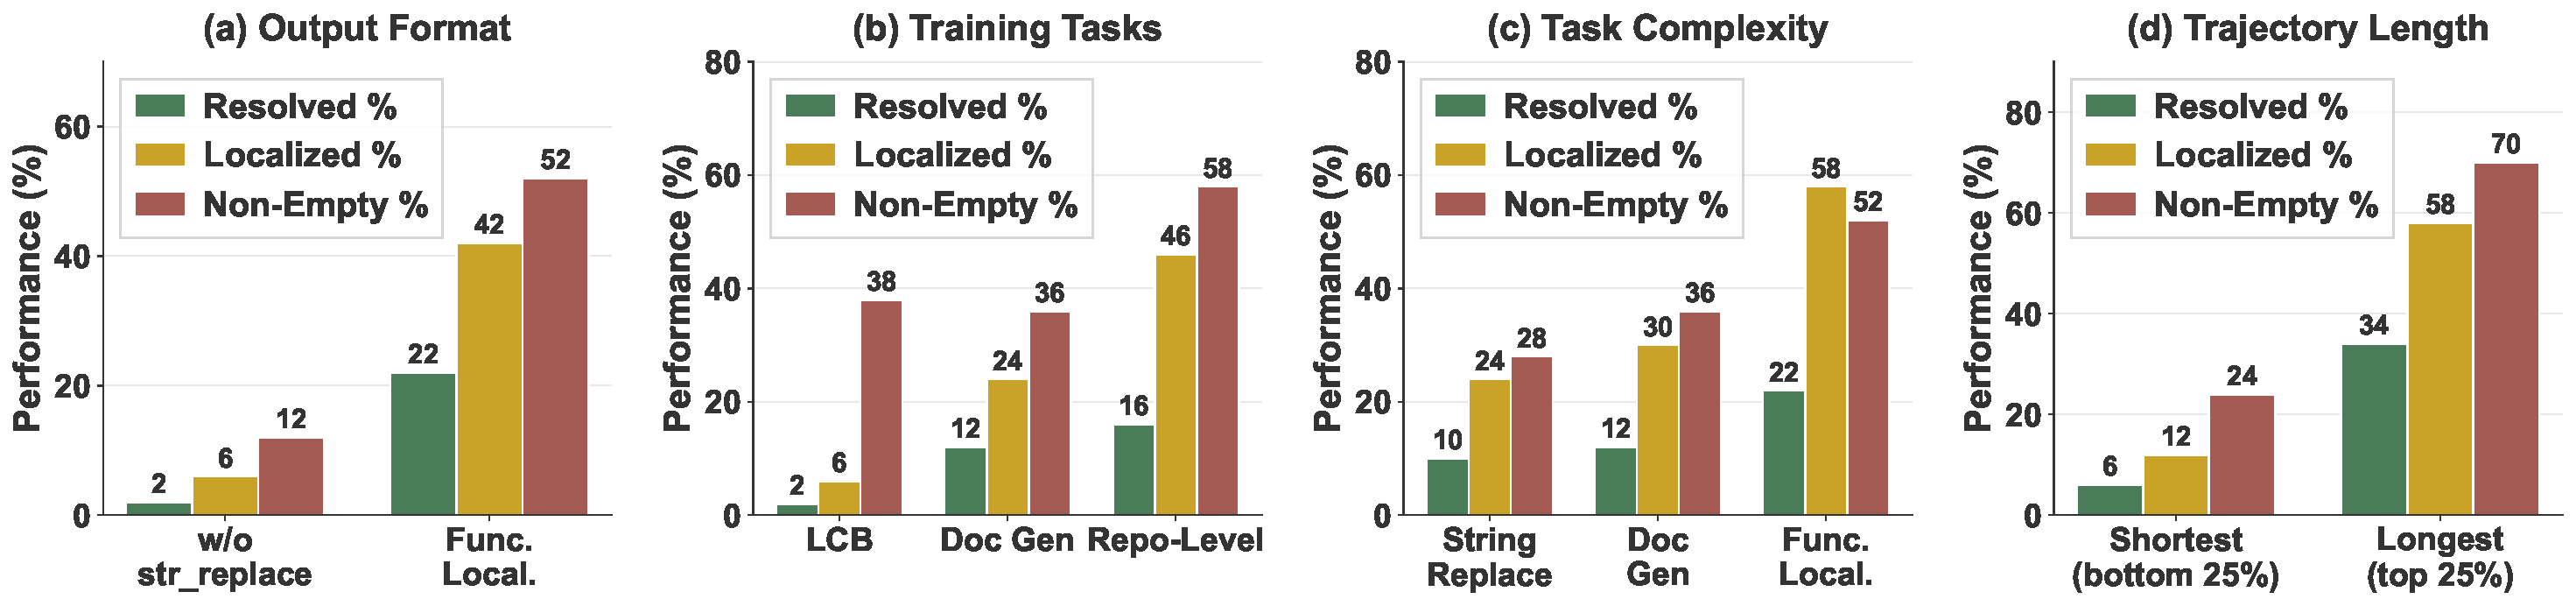
\includegraphics[width=\textwidth]{HybridGym_figs/fig_combined_bcde.pdf}
\caption{Controlled experiments on training data characteristics.
(a)~\textbf{Output Format:} Removing the file editing actions (\texttt{str\_replace}) from function localization trajectories causes a large drop in SWE-bench resolution rate.
(b)~\textbf{Repo-Exploration:} script-level code generation (LCB) does not effectively transfer to repo-level issue-solving and even underperforms documentation generation, a simple repo-level task.
(c)~\textbf{Task Complexity:} Transfer improves as training tasks become more complex.
(d)~\textbf{Trajectory Complexity:} With a fixed data size, training on longer (more agent steps) trajectories substantially improves downstream performance.}
\label{fig:ablation}
\end{figure*}







\section{Analysis of Task Transferability}
\label{sec:controlled-exp}

We have established in \S\ref{sec:exp} that the particular tasks included in \repostmethodname are effective for task generalization across diverse real-world coding benchmarks. 
In this section, we investigate: \textbf{what properties of these trajectories enable task transfer?}
To answer this, we run controlled ablations that systematically modify trajectory structure and measure the resulting changes in performance.

As the ablations require repeated evaluation across many variations, we keep the analyses computationally tractable by evaluating on an easier subset of SWE-bench examples (denoted as ``Easy 50''), which are solvable by Deepseek-v3, a strong reference model \cite{deepseekv3}. 


\subsection{Output Format Must Match Downstream Tasks}
While our tasks are designed around higher level tasks such as function localization and generation, we also find that \textit{how} these behaviors are expressed in the training trajectories matters. Specifically, as stated in [\textbf{Principle 1}] in \S\ref{sec:methodology}, we find that the output format of the tasks is a crucial factor.

All three downstream tasks in our experiments require the agent to generate a code patch as the output. To isolate the role of output format, we conduct a minimal ablation on our function localization task: instead of requiring the model to generate a comment in the codebase containing the fix plan, we simply ask it to generate the plan in a message.
We accordingly modify the training trajectories by removing the \texttt{str\_replace} actions for writing comments and adding the fix plan in the final message generated by the agent.

As shown in \autoref{fig:ablation}, performance on SWE-bench collapses when we remove the string replacement actions. These results suggest that for coding agent tasks, the production of \textbf{patch-like outputs} is not a superficial formatting choice but a crucial skill that the agent needs to learn. 


\subsection{Script-level Agentic Tasks Do NOT Generalize to Repo-level Tasks}
\label{sec:ablation_lcb}
We then validate [\textbf{Principle 2}], which requires the training tasks to have a repo-exploration stage. 
To test this, we implement a script-level task, LiveCodeBench (LCB) \cite{livecodebench}, which primarily evaluates function generation in a single file. 
We contrast it with two repo-level tasks: 
(1) the repo-level function generation task we use in \repostmethodname (introduced in \S\ref{sec:methodology}), and 
(2) documentation generation, which requires the agent to generate the docstring for a given function.
For fair comparison, we wrap the coding template and test script in LCB in a dummy repository so that the model interacts with the same harness and tool API. 


\autoref{fig:ablation} shows that despite having the wrapper to make LCB superficially a repo-level task, LCB is not effective for transfer to SWE-bench. 
This negative result suggests that repository-level generalization requires more than superficial ``agentic formatting.'' 
In particular, repo-level tasks induce behaviors that are largely absent from script-level problems: identifying and navigating relevant files, grounding edits in existing codebase structure, and producing concrete patch-like modifications that apply cleanly in context. 



\begin{figure}[t]
\centering
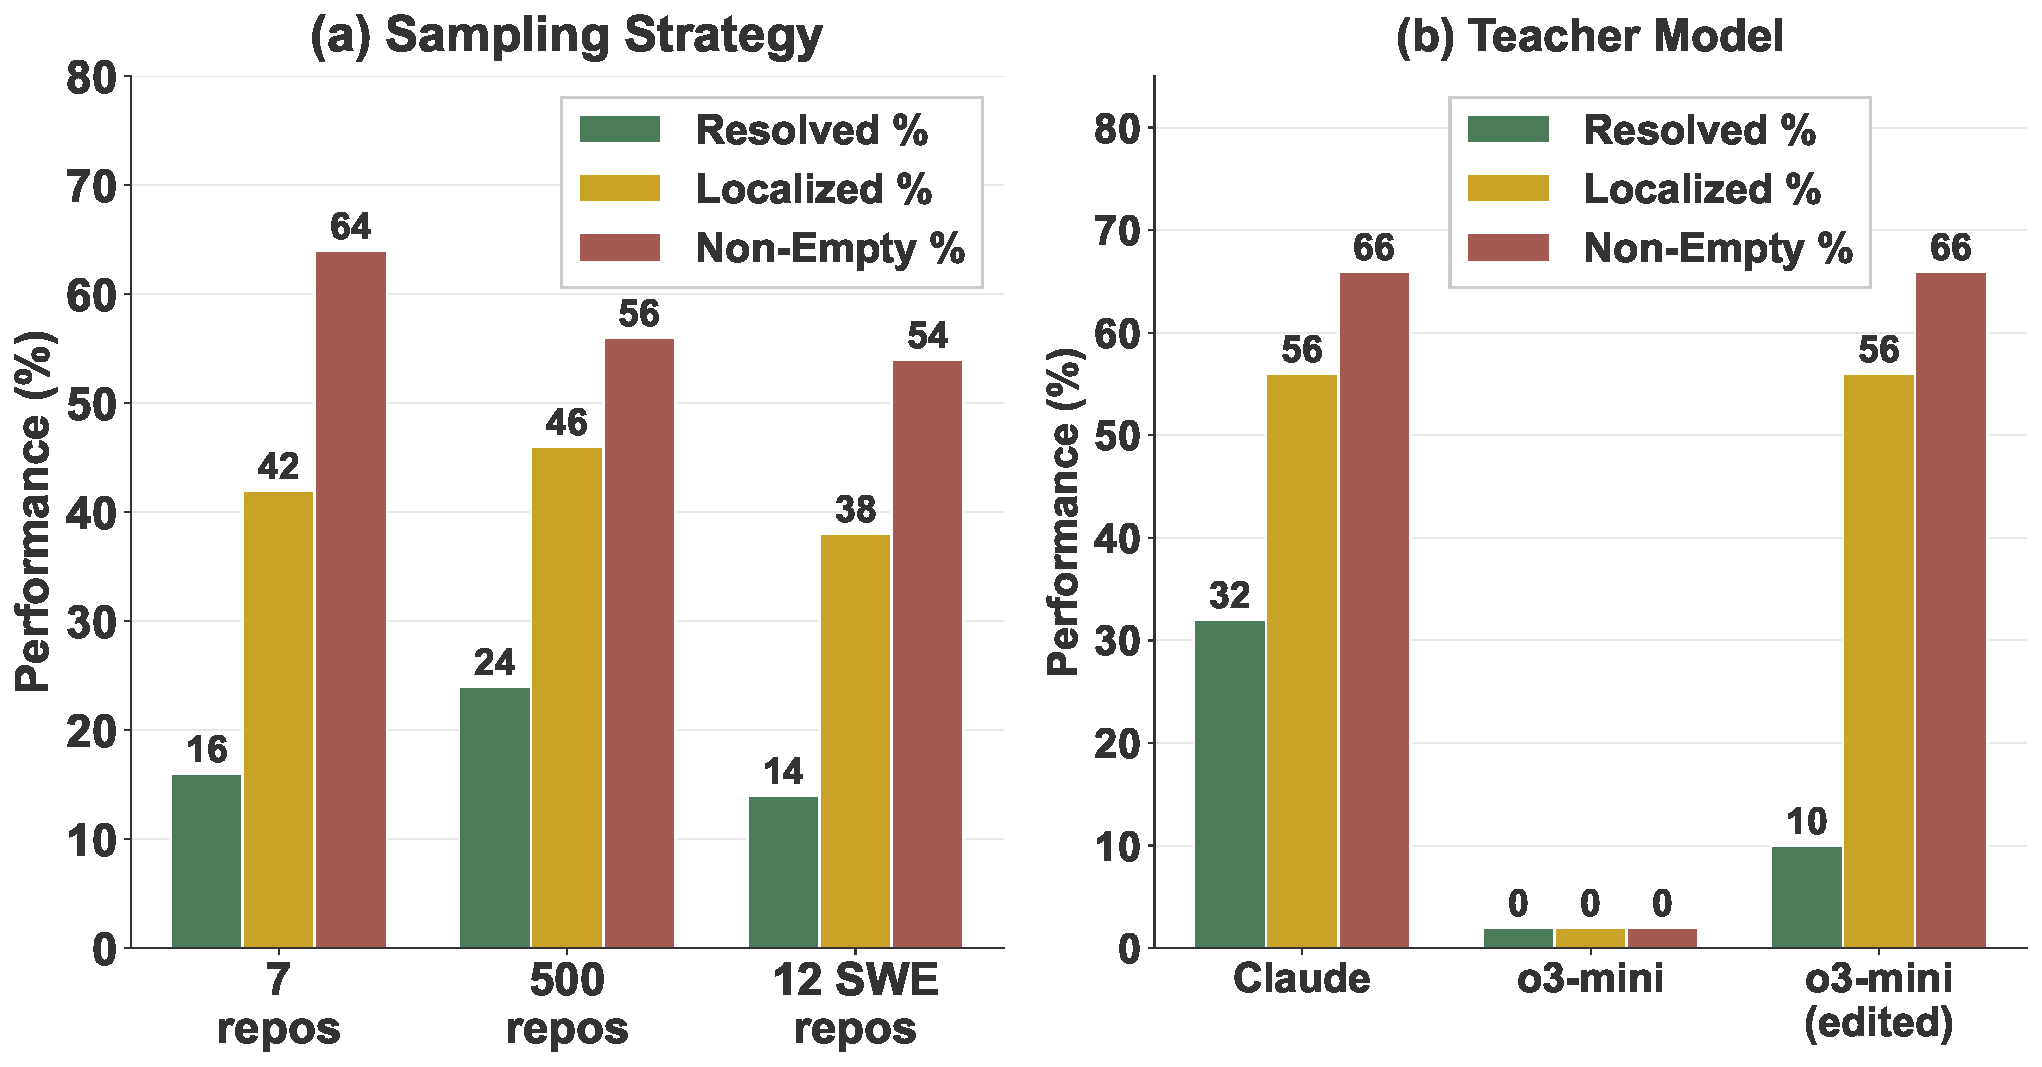
\includegraphics[width=0.7\columnwidth]{HybridGym_figs/fig_sampling_teacher_combined.pdf}
\caption{Effect of teacher model and data selection. (a) Effect of \textbf{sampling strategy} at fixed training budget. Repository diversity improves training but using the same repositories as in evaluation does not. 
(b) training on issue localization trajectories with different \textbf{teacher models}. o3-mini (edited) indicates the same set of trajectories as o3-mini, but with text and action steps combined. 
}
\label{fig:sampling_teacher}
\end{figure}

\subsection{Task and Trajectory Complexity Matters}
\label{sec:ablation_complexity}
After identifying reasoning and planning as a crucial component in coding tasks in \S\ref{sec:methodology}, we derive [\textbf{Principle 3}] that requires the task to involve a non-trivial level of reasoning.
Here, we examine whether task generalizability improves as training supervision more closely matches the multi-step, tool-mediated interaction patterns required for coding tasks. 

We first examine tasks with ascending complexity: (1) single-shot string-replacement edits in which the task is to refactor a function by simply renaming it without replacing other usages of it, (2) documentation generation for a fixed function (as in $\S\ref{sec:ablation_lcb}$), and (3) the function localization task, which requires more complex reasoning than the previous two tasks.
We see in \autoref{fig:ablation} that as tasks become more complex and interaction-heavy, downstream SWE-bench performance improves, and models are substantially more likely to produce non-empty patches.


To isolate complexity effects from task identity, we also investigate the effect of \emph{trajectory complexity}, which is operationalized as the number of agent actions (tool calls and intermediate components) taken in successful trajectories.
We pool trajectories from our repo-level task mixture and partition them by length, selecting the shortest and longest quartiles (25\% each). 
As shown in \autoref{fig:ablation}, although the training sizes are the same, training on longer trajectories yields a large improvement in SWE-bench resolution rate, alongside a sharp reduction in empty generations. These results suggest that trajectory complexity is an important driver of task performance.



\subsection{Even Successful Trajectories of the Same Task Instances may have Different Impact}
In addition to training task design, we observe that \textbf{the teacher model also plays a crucial role in effective training}.
Specifically, we find that even successful trajectories for the same instances can yield very different distillation outcomes.
We illustrate a particular case in \autoref{fig:sampling_teacher}. 
On the issue localization task, we found that distilling from Qwen3-235B and Claude trajectories transfers well to SWE-Bench, but distilling from o3-mini trajectories degrades student performance. 
The key difference we found is that o3-mini frequently separates reasoning and actions (i.e., tool calls) into different turns.
After training on such data, the agent collapses to the distribution of thinking-only conversational turns and does not learn to call tools at all.
We edit o3-mini trajectories by simply stitching adjacent rationale and action steps into a single example. The resulting data effectively transfers to SWE-Bench, indicating that model-specific behaviors such as separating reasoning and actions can strongly influence the effectiveness of distillation.


\subsection{Sampling Strategies Affects Effectiveness}
Finally, beyond task choice and trajectory structure, we also find that how training instances are sampled impacts downstream transfer. 
We examine two key factors: 
(1) repository diversity (i.e., the number of repositories covered by the training set), which is identified by previous works~\cite{repost,swe-smith}, and 
(2) the domain of code. In the extreme case, we build training data from the exact same repositories we use in evaluation.

To investigate this, we keep the training budget fixed at 500 trajectories and sample from function localization trajectories. We compare:
(i) \emph{Min Repo-Diversity}, where we aggregate instances from a small number of large repositories (7 repositories), 
(ii) \emph{Max Repo-Diversity}, where we sample one instance per repository (500 repositories) to maximize repository coverage, and 
(iii) \emph{In-Domain Repos}, where we construct function localization trajectories based on the 12 SWE-Bench repositories.

Despite using the same number of training instances and the same SFT recipe, \emph{Max Repo-Diversity} yields higher SWE-bench resolution (\autoref{fig:sampling_teacher}). 
This suggests that exposure to a broader range of repository structures improves generalization to unseen repositories.
Surprisingly, \textbf{training on the same repositories in evaluation does not improve the performance}, suggesting that learning general agent skills is more crucial than memorizing repo-specific information.




% \section{Related Work}
% \start{Coding Agents}
% Compared to traditional seq-to-seq code generation~\cite{codex} or static pipelines~\cite{agentless,swe-search}, coding agents can dynamically call tools to interact with the environment, enabling end-to-end problem solving.
% Recent works develop various coding agent scaffolds, including SWE-Agent~\cite{sweagent}, Live-SWE-agent~\citep{live-swe-agent} and OpenHands~\cite{openhands}
% Such agentic methods achieve strong performance on diverse coding benchmarks, including issue-solving~\cite{swebench} under various settings~\citep{swebench,swebench-pro,swebench-multimodal,multi-swe-bench}, test generation~\cite{swt-bench,testgeneval}, and feature construction~\cite{commit0,repocoder,R2E,codebenchgen,kernelbench}.
% We therefore focus on improving agent systems for coding tasks.

% \start{Coding Agent Pre-training}
% In the pre-training stage, recent work train the language models on general agentic tasks, including proprietary models~\cite{gpt5,claude45} and open-sourced ones~\cite{qwen3,deepseekv3}.
% For instance, Kimi-K2~\cite{kimik2} constructs a wide range of synthetic tools and tasks to boost general agentic abilities.
% In this work, we focus on synthetic tasks for coding agents.

% \start{Coding Agent Post-training}
% In the post-training stage, one line of work focuses on the training method, such as rejection sampling~\cite{swegym} and reinforcement learning~\cite{swerl,rlcoder,mlagent}.
% Another line of work improves training data construction, yet most prior datasets only cover a single task such as issue-solving~\cite{swegym,swefixer,swegpt,R2EGym,swe-smith}, neglecting other crucial applications, including test generation and library construction.
% A concurrent work, SWE-Play~\cite{swe-play}, designs training data for each of the downstream tasks and additionally presents agent-proposed tasks. 
% However, they do not conduct in-depth analysis on task transferability and fully rely on the agent to set up the complicated training environments, including building and installing a repository from scratch, which is challenging and limits the scalability.
% In contrast, we conduct systematic analyses on what transfers and what does not for coding tasks and design scalable and cost-efficient tasks based on analysis results.






\section{Chapter Summary}
In this chapter, we improve the task transferability of coding agents. 
We conduct in-depth analyses of the transferability across coding agent tasks.
We find that there are similar components shared by diverse real-world coding tasks (e.g., repo-exploration) that can be achieved by the agent with similar commands.
Based on the discovery, we derive a set of principles for task design, including output format matching, requiring repo-exploration, non-trivial reasoning, and simple setup.
We present four scalable and cost-efficient tasks that do not require setting up executable repositories.
With the resulting dataset, \repostmethodname, we achieve strong task generalization results on three real-world benchmarks. For instance, even without issue-solving or test-generation data in training, we improve Qwen2.5Coder-32B by 25.4\% on SWE-Bench Verified and 7.9\% on SWT-Bench Verified.
We also improve existing in-domain datasets by combining them with \repostmethodname (e.g., improving SWE-Play by 4.9\% on SWT-Bench Verified).

The principles introduced in this chapter focus on training task design. However, as studied in \S\ref{sec:controlled-exp}, there are other aspects that are also crucial for agent training, such as training instance selection and the concrete actions in successful training trajectories.
We thus propose \autoref{chap:effective-analysis} to investigate more training data construction principles, focusing on the effectiveness of training trajectories.































\chapter{On the Agent Behaviors that Generalize across Coding Tasks \textcolor{mediumgreen}{(\textit{proposed})}}
\label{chap:effective-analysis}



\section{Introduction}
\label{plus:sec:introduction}
In \autoref{chap:hybrid-gym}, we introduce Hybrid-Gym~\cite{hybrid-gym}, which trains a general-purpose coding agent by deriving a set of training task design principles. 
However, \textbf{having proper training tasks is not the only condition for effective coding agent training}.

In addition to training tasks, both Hybrid-Gym and previous work discover other crucial factors of the training outcome.
With rejection sampling finetuning as the training paradigm~\cite{rejection-sampling}, SWE-Gym~\cite{swegym} and SWE-Smith~\cite{swe-smith} find that training instances with a balanced difficulty distribution improve training results.
RepoST~\cite{repost}, SWE-Smith~\cite{swe-smith}, and Hybrid-Gym~\cite{hybrid-gym} demonstrate that it is beneficial to cover diverse repositories in the training data.
Hybrid-Gym~\cite{hybrid-gym} shows that training on trajectories with more steps improves performance.

\begin{table}[t]
  \centering
  \small
  \resizebox{\columnwidth}{!}{%
  \begin{tabular}{l ccc}
  \toprule
  \multirow{2}{*}{\bf Teacher Model (|Train Size|)} &
  \multicolumn{3}{c}{\bf SWE-Bench Verified (Easy 50)} \\
  \cmidrule(lr){2-4}
  & Resolved \% & Localized \% & Non-Empty \% \\
  \midrule
  \sdlrow & \multicolumn{3}{c}{\textit{Base Model: Qwen2.5Coder-7B}} \\
  \midrule
  \textemdash & \worse 2.0 & 4.0 & 8.0 \\
  \midrule
  Qwen2.5Coder-32B (400) & \bad 4.0 & 20.0 & 48.0 \\
  Qwen2.5Coder-32B (Advanced Prompt) (400) & \good 8.0 & 46.0 & 68.0 \\
  Claude-Sonnet-3.7 (400)   & \better \bf 26.0 & 68.0 & 86.0 \\
  \bottomrule
  \end{tabular}%
  }
  \caption{Results on training Qwen2.5Coder-7B on successful trajectories of the exact same 400 function localization instances generated by Claude-3.7, Qwen2.5Coder-32B, and Qwen2.5Coder-32B with the more detailed prompt we develop in the preliminary experiments (denoted as Advanced Prompt). 
  We evaluate the student models on a subset of the SWE-bench Verified issue-solving dataset after training. 
  }
\label{ablation:self-vs-claude}
\end{table}

In this chapter, we show that beyond task success, the specific agent behaviors in the training trajectories substantially affect the effectiveness of training, and \textbf{we aim to discover and verify the particular agent behaviors that affect training effectiveness, for both in-domain and task-transfer training}. Our study provide insights into why and how task generalization can be achieved for coding agents. Furthermore, our study provides guidelines for the construction and selection of training data before running the training.

In our \textcolor{aquablue}{\textbf{preliminary experiments}}, as shown in \autoref{ablation:self-vs-claude}, we use a frontier model (Claude-Sonnet-3.7) and a weaker model (Qwen2.5Coder-32B) to generate successful trajectories on the exact same set of 400 function localization instances and distill Qwen2.5Coder-7B.
We can see that distilling from Claude-Sonnet-3.7 achieves a substantially higher performance.

We first discover the differences between the two models' successful trajectories. Inspired by existing research that extract agent behavior patterns in general domains~\cite{beneficial-reasoning}, we use an LLM agent to discover the differences, with the two models' successful trajectories as context.
After manually examining the LLM agent's output, we observe that although both models succeed on the task, Claude-3.7 adopts a more systematic repo-exploration strategy. For instance, it first narrows down the candidate files to a limited number, and then locates relevant functions inside the candidate files by keyword searching. In contrast, Qwen2.5Coder-32B typically locates functions by directly reading the entire candidate file instead of keyword searching, which could be very inefficient when the file is large.

We then verify that one of the key behaviors we found: using keyword searching to locate functions inside files, is indeed beneficial for training.
In particular, we add a more detailed repo-exploration instruction to the prompt for generating training trajectories. We then generate 400 successful trajectories with Qwen2.5Coder-32B and compare the distillation performance with the original prompt.
As shown in \autoref{ablation:self-vs-claude}, we observe that (1) the distillation performance is improved from 4.0\% to 8.0\% with the new prompt, and (2) the model distilled from the new prompt also generates more keyword searching actions when localizing code inside files.

Our preliminary experiments show that we can discover important agent behaviors that affect distillation performance by first discovering candidate agent behaviors based on the differences between two teacher model's successful trajectories, and then verifying their importance by conducting controlled experiments.
However, our preliminary experiments have three \textbf{limitations}: 
(1) the discovery of key behaviors is still challenging for the agent, which requires extracting patterns from the entire trajectories that contain 20-30 steps on average,
(2) prompt engineering is not always effective to control the presence of particular agent behaviors -- it also depends on whether the model can follow the instruction correctly, and we may need to carefully tune the prompt, and 
(3) the analysis is conducted on only one particular teacher model pair and one training task.

To address the limitations, we \textcolor{mediumgreen}{\textbf{propose}} a more comprehensive analysis. In particular,

\noindent(1) To make candidate agent behavior discovery easier, we categorizes behaviors into stage-level, stage-strategy-level, and step-level behaviors based on whether they are about high-level strategies or concrete steps. We provide different types of context to the LLM agent to discover the behaviors at different levels.

\noindent(2) To make the presence of particular agent behaviors in trajectories more controllable, we propose trajectory editing methods that adds or removes a target behavior from the training trajectories.
We propose a list of rules to describe conditions where we can alter steps in a trajectory without breaking the trajectory's consistency.
If trajectory editing is not trivial for some behaviors, we fallback to the prompt engineering and data filtering method, as introduced in the preliminary experiments.
Finally, similar to the preliminary experiments, we train a student model on the original and edited trajectories and compare the distillation performance.

\noindent(3) We extend the analysis to multiple training tasks and multiple teacher model pairs. We keep a global list of important agent behaviors and update the list whenever we add a new analysis setting. The analysis of multiple teacher models enables us to have a more comprehensive list of key agent behaviors. The analysis of multiple training tasks reveals agent behaviors that are transferable across different tasks.



\begin{table}[t]
  \centering
  \small
  \resizebox{\columnwidth}{!}{%
  \begin{tabular}{l ccc}
  \toprule
  \multirow{2}{*}{\bf Features} &
  \multicolumn{3}{c}{\bf Training Data (Function Localization)} \\
  \cmidrule(lr){2-4}
  & Qwen-32B & Qwen-32B (Advanced Prompt) & Claude-3.7 \\
  \midrule
  \# of In-file Search Actions & \bad 0.34 & \better 1.73 & \better 1.62 \\
  \bottomrule
  \\
  \toprule 
  \multirow{2}{*}{\bf Features} &
  \multicolumn{3}{c}{\bf SWE-Bench Verified (Easy 50)} \\
  \cmidrule(lr){2-4}
  & Student of Qwen-32B & Student of Qwen-32B (Advanced Prompt) & Student of Claude-3.7 \\
  \midrule
  \# of In-file Search Actions & \bad 1.57 & \good 2.10 & \better 7.30 \\
  \bottomrule
  \end{tabular}%
  }
  \caption{Frequency of infile keyword searching actions in the training trajectories of Qwen-32B and Claude-3.7 and the evaluation trajectories of their student models. We observe that the student models inherit the teacher's strategies in training trajectories.}
  \label{tab:plus:prelim1}
\end{table}





\section{Overview of Proposed Methods}
The main motivation of this project is to reveal what exact agent behaviors are important for the effectiveness of coding agent training, for both in-domain and task-transfer training.

The proposed methdos consist of two parts: (1) \textbf{discovery} of candidate agent behaviors that could potentially affect performance by finding the differences between these two models' successful trajectories, and (2) \textbf{verification} of the importance of these behaviors by conducting controlled experiments to reveal their effects on distillation performance.

The proposed framework that aims to address the limitations mentioned in \autoref{plus:sec:introduction} is as follows:
for the discovery part (\autoref{plus:sec:categorization}), we categorize agent behaviors based on whether they are about high-level strategies or concrete steps. When we apply an LLM agent to discover the behaviors at different levels, we provide different types of context to the agent.
The agent iteratively discovers new candidate behaviors based on the differences between the frontier and weaker teacher model's successful trajectories, examines whether the behaviors are well-defined and distinguishing, and discover new candidate behaviors.
For the verification part (\autoref{plus:sec:controlled-exp}), for each candidate agent behavior, we conduct controlled experiments by editing the training trajectories to add or remove the behavior. We provide a list of rules to describe conditions where we can edit trajectories without affecting its validity. We then compare the distillation performance on the original and edited trajectories to assess the importance of the behaviors.
We prioritize the candidate behaviors that are directly related to the key outcome of the task (e.g., the final code patch and the function and file it locates for the issue-solving task).
We iteratively perform the discovery and verification processes until we cannot find any new candidate agent behaviors.

Finally, we further extend the analysis to multiple teacher model pairs and multiple coding agent training tasks to obtain a more comprehensive list of important agent behaviors that affect distillation performance (\autoref{plus:sec:extend-exp}).


\begin{figure}[t]
  \centering
  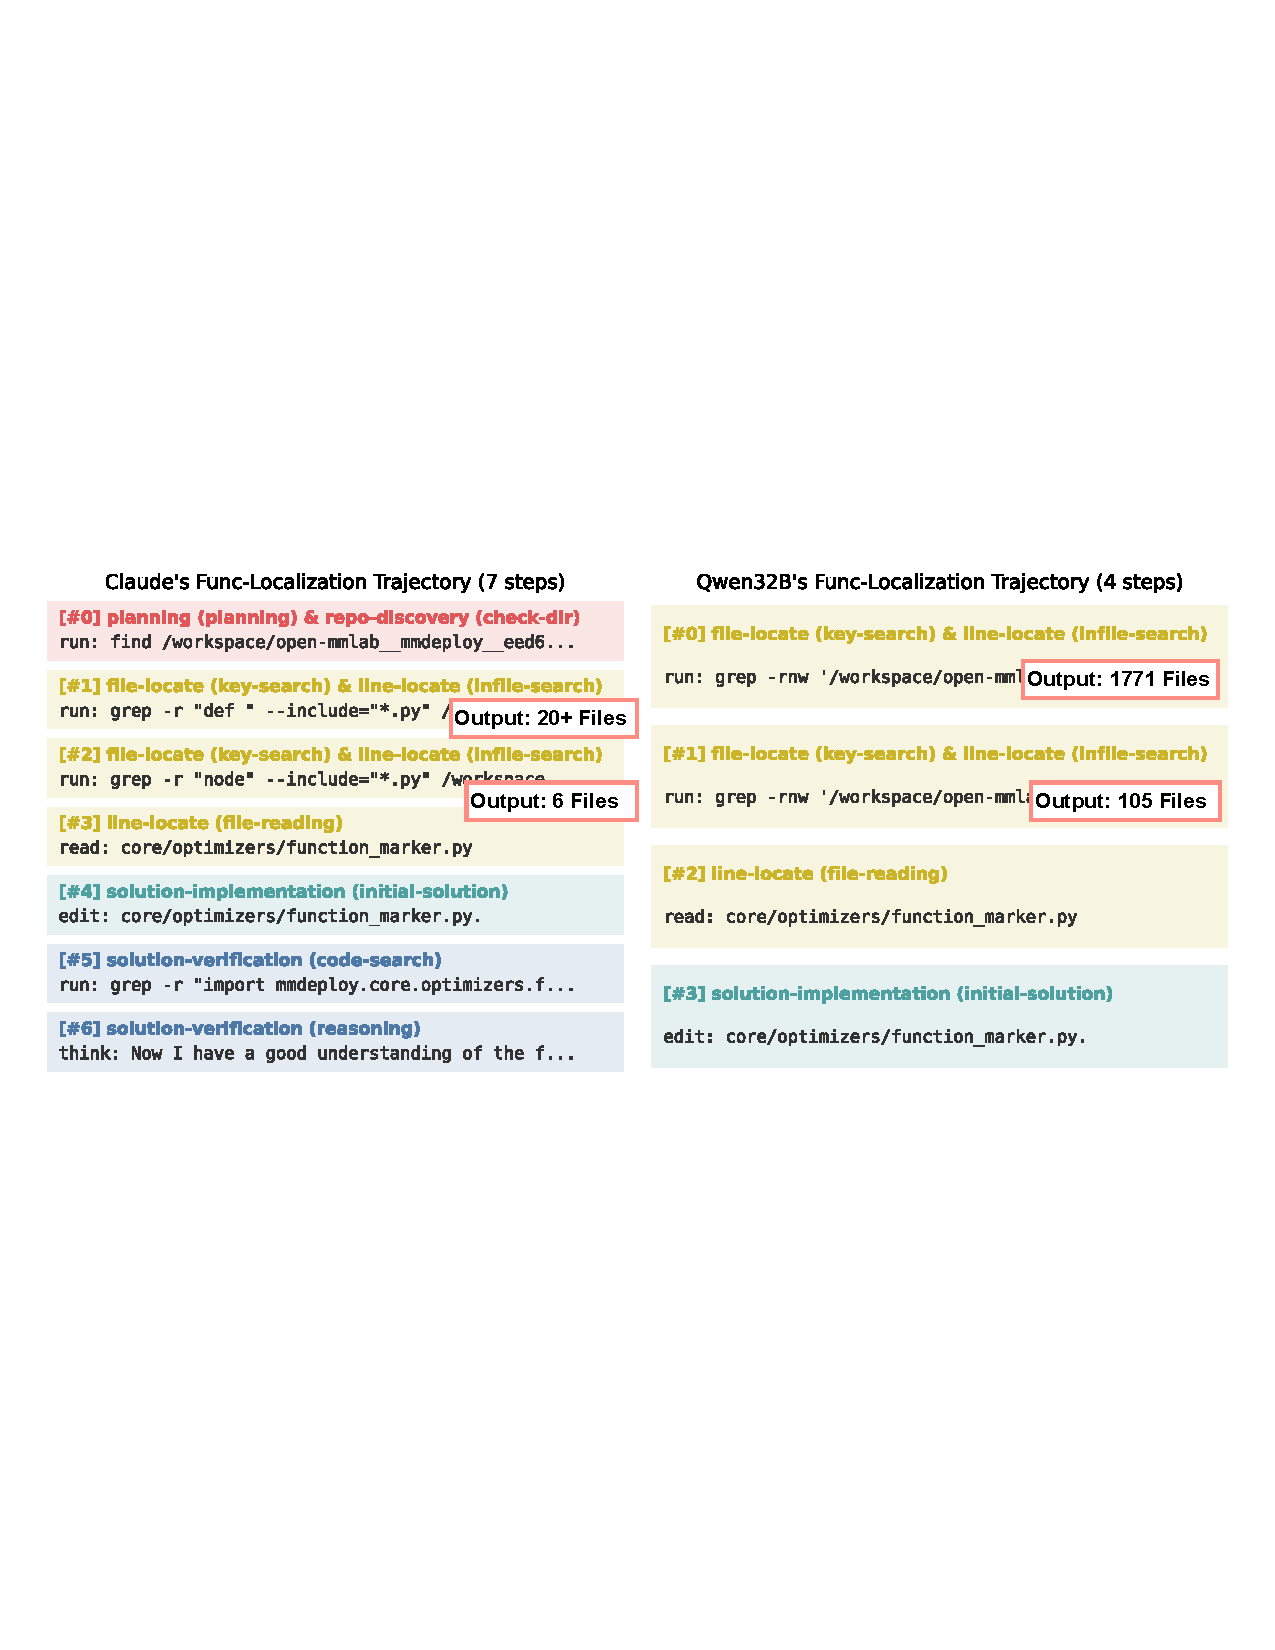
\includegraphics[width=\columnwidth]{plus_figs/trajectory_comparison.pdf}
  \caption{An example of how we represent trajectories at different abstraction levels. We show the categorization of each agent step in the format of ``stage label (strategy label)''. Note that the agent step can be categorized into multiple stages and strategies.}
  \label{fig:plus:abstraction}
\end{figure}


\section{Proposed Method 1: Candidate Agent Behavior Discovery for Different Abstraction Levels}
\label{plus:sec:categorization}
\subsection{Proposed Method}
Previous work and our preliminary experiments discover candidate agent behaviors by presenting the entire successful trajectories generated by two teacher models as context to an LLM agent and prompting it to discover different behaviors, which is still challenging for the agent.
Towards this challenge, our key intuition is that agent behaviors arise at different abstraction levels, and discovering them does not always require access to the full trajectory.
For example, we only need the high-level summary of the trajectory to identify whether an agent repeatedly performs verification after implementation.
Another example is that to compare the strategy used by the agent to localize a function, we only need to look at the function localization steps rather than the entire trajectory.

In summary, we categorize agent behaviors into three abstraction levels: \textbf{stage-level}, \textbf{stage-strategy-level}, and \textbf{step-level}, which enables us to design different types of context for the LLM agent to discover the behaviors at different levels.


\start{Represent Trajectories at Different Abstraction Levels}
The categorization of agent behaviors is based on how we represent each agent step at different abstraction levels.
In particular, we define:
\begin{itemize}
  \item \textbf{The Stage of Coding Tasks}: Build upon the analysis of Hybrid-Gym~\cite{hybrid-gym}, we pre-define the stages that are shared across different coding tasks: planning, repository discovery (e.g., checking the structure of the repository), file localization, code-line localization, code reproduction, solution implementation, and solution verification. Based on the analysis in Hybrid-Gym, the stages are shared across three downstream coding tasks: issue-solving, test generation, and library construction, and four synthetic training tasks: function localization, issue localization, dependency search, and function generation.
  \item \textbf{The Strategy to Complete a Stage}: For each stage, we define the strategy to complete the stage, or equivalently, the purpose of each action that is used to complete the stage. For instance, for the code-line localization stage, the strategy includes searching for keywords inside candidate files, reading the candidate files, executing relevant code and observing the error message, etc.
\end{itemize}

As shown in \autoref{fig:plus:abstraction}, given a set of trajectories, we assign a stage label and a strategy label to each agent step. 
We iteratively update the categories when we conducting new analyses and discovering new agent behaviors.
We keep adding new stages or strategies if we find agent steps that are not covered by the existing categories.
We can also break down a category into smaller categories if we find that it is too broad.



\start{Agent Behaviors at Different Abstraction Levels}
We categorize the agent behaviors based on which abstraction level of trajectory they are be represented at.
\begin{itemize}
  \item \textbf{Stage-level Behaviors}: the presence, order, or transition of different stages in the trajectory.
  For example, as shown in \autoref{fig:plus:abstraction}, Claude-3.7 has a ``solution verification'' stage after ``solution implementation''.
  % transits from the ``file localization'' stage to the ``function localization'' stage only when the number of candidate files is reduced to a limited number.
  \item \textbf{Stage-strategy-level Behaviors}: the presence, order, or transition of different strategies to complete a particular stage.
  For example, as shown in \autoref{fig:plus:abstraction}, for the function localization stage, Claude-3.7 performs several keyword searching actions that present both the file and the located lines of code. Then it perform file-reading actions to read the corresponding lines.
  \item \textbf{Step-level Behaviors}: properties of the specific messages generated by the agent. For instance, the agent correctly uses the ``file-editing'' tool to generate code patches with no errors and retries. Another example is that the agent generates long reasoning before generating the actions.
\end{itemize}

Note that in Hybrid-Gym~\cite{hybrid-gym} (\autoref{chap:hybrid-gym}), we present three principles for effective task design: (1) the tasks should generate a code patch as the outcome, (2) the tasks should involve a meaningful repository-exploration phase, and (3) the tasks should require non-trivial reasoning.
All the three principles can be translated to the agent behaviors with our definition: (1) the trajectory contains the ``solution implementation'' stage, (2) the trajectory contains the ``repository discovery'', ``file localization'', or ``code-line localization'' stages, and (3) the trajectory contains the ``planning'' stage, which are all stage-level behaviors. In this study, we conduct a more comprehensive analysis by including behaviors from all the three levels.


\start{Discovering Candidate Agent Behaviors at Different Abstraction Levels}
Similar to the preliminary experiments, we use an LLM agent to discover different agent behaviors in the two sets of trajectories.
In addition to access to the entire trajectories, we provide different context for the discovery of behaviors at different levels.
For stage-level behaviors, we provide the trajectories that are abstracted with the stage labels.
For stage-strategy-level behaviors, we provide the steps in the trajectories that belong to a particular stage. We additionally provide the strategy labels of these steps.
For step-level behaviors, we do not provide additional context other than the full trajectories, but we explicitly prompt the LLM agent to focus on the content of the single step.

The agent iteratively discovers new candidate behaviors based on the differences between the frontier and weaker teacher model's successful trajectories, examines whether the behaviors are well-defined and distinguishing, and discovers new candidate behaviors.


\subsection{Proposed Experiments}
We follow the preliminary experiments and compare the trajectories generated by a frontier and a weaker teacher model (e.g., Claude-3.7 and Qwen2.5Coder-32B). We start with training on the function localization task and evaluating on the SWE-Bench Verified issue-solving dataset. We will then extend the analysis to multiple teacher model pairs and multiple coding agent training tasks, which will be introduced in \autoref{plus:sec:extend-exp}.

Since the goal is to discover the agent behaviors that lead to the different distillation performances, we examine the two properties of each candidate agent behavior we discover: (1) Well-defined. (2) Distinguishing.

\start{Verification of Well-defined Agent Behaviors}
An agent behavior is well-defined if there exists a deterministic method to determine whether a trajectory contains the behavior. Furthermore, the behavior can be represented by a binary feature. For instance, the agent behavior ``using keyword searching to locate functions inside files'' is well-defined, but the agent behavior ``has comprehensive repository exploration'' is not, because it is ambiguous and does not have a precise operational definition.

For each candidate behavior, we use an LLM-based annotator to determine whether the behavior is present in a trajectory. The annotator outputs one of three labels: \texttt{present}, \texttt{absent}, or \texttt{unable\_to\_determine}. The annotation prompt includes the behavior definition and the formatted trajectory. To reduce annotation noise, we use a fixed prompt template and keep the annotator model unchanged across all experiments. 
We additionally validate the LLM annotations based on its agreement with human annotations on a small subset of trajectories.

To verify whether a candidate agent behavior is well-defined, we randomly sample $k$ instances where both of the two teacher models generate a successful trajectory, and apply the LLM-based annotator to all of the $2k$ trajectories. We compute the rate of \texttt{unable\_to\_determine} outputs for that behavior. We only retain behaviors whose indeterminate rate is below a threshold $\tau$ (e.g., $5\%$).


\start{Verification of Distinguishing Agent Behaviors}
To verify whether an agent behavior is distinguishing, similar to the above experiment, we randomly sample $k$ successful trajectories from each of the two teacher models and apply the LLM-based annotator to all of the $2k$ trajectories.

For each well-defined behavior, we define a binary feature for each trajectory: 1 the behavior is present in trajectory, and 0 otherwise.
We then test whether the prevalence of this behavior differs significantly between the two teacher models. Since this feature is binary, we use a chi-square test as the statistical test. 

Specifically, we construct a $2 \times 2$ contingency table over \{teacher model A, teacher model B\} and \{behavior present, behavior absent\}, and compute a p-value for the null hypothesis that the behavior occurs at the same rate in both models. We retain behaviors with a p-value below a threshold $\delta$ (e.g., $0.05$).



\section{Proposed Method 2: Controlled Experiments based on Trajectory Editing}
\label{plus:sec:controlled-exp}
\subsection{Proposed Method}
The goal of this part is to verify whether particular agent behaviors affect distillation performance.
A main limitation of the preliminary experiments is that, even if we prompt the teacher model to exhibit or avoid a target behavior, the model may not reliably follow the instruction. 

To address this limitation, we propose to conduct controlled experiments by directly editing the training trajectories to add, remove, or modify a target behavior whenever such editing is feasible.

The key intuition behind trajectory editing is that we only focus on trajectories that \emph{successfully} solve the task.
If an agent successfully solves the task, it is also likely to produce the \emph{essential intermediate outcomes} when completing the task.
For example, in the function localization task, where the agent must identify a target function from its description and generate a docstring for it, it is likely that the agent sees the target filename and the function content in some of the action outputs, and there must exist a step that edits the target function.
This observation makes it possible to edit some behaviors locally while preserving the overall consistency of the problem-solving process, as long as the edited part is producing the same essential intermediate outcome.
In other words, trajectory editing is suitable for behaviors that do not alter the essential intermediate outcome, but only changes \emph{how} the agent reaches or expresses that outcome.



\start{Principles of Trajectory Editing}
The main challenge of trajectory editing is to ensure that the edited trajectory remains \emph{consistent}. Here, consistency means that the edited trajectory still constitutes a valid successful problem-solving process, where (1) at least one step must still produce the final task outcome (e.g., a code patch that satisfies the task requirements), and (2) each step must have sufficient information from the previous context to justify its action.

We define a set of rules describing when trajectory steps can be added, removed, or modified without affecting the trajectory's consistency:
\begin{itemize}
    \item \textbf{Equivalent step substitution.} If two sets of agent steps require the same context and produce the same essential intermediate outcome, then one can be substituted for the other without affecting trajectory consistency. For example, in the file localization stage, the agent may perform search with different keywords. As long as target file appears in the search results, we can substitute the search steps.
    
    \item \textbf{Removal of non-essential steps.} Steps that do not provide necessary information for any subsequent step can be removed. Examples include file-search actions that do not lead to relevant results, verification of the generated code patch after it is already applied, or any actions that are failed to applied because the syntax is incorrect. 
    Note that removing such steps may make some later actions appear less well-motivated or less sound, but the trajectory still remains consistent.
    
    \item \textbf{Editing textual content.} The textual content of a step can be modified as long as the revised content remains consistent with the previous context. The reason is that only the action generated by the agent will be executed, and the execution output is not affected by the textual content.
    For instance, an action rationale may be rewritten to be more concise, or a message may be rephrased without changing the information it conveys.
\end{itemize}

We would like to note that these rules serve as an initial set of editing principles rather than a complete characterization. 
As the project progresses, we will introduce additional editing rules when new trajectory patterns and edge cases are identified.





\start{Examples of Controlled Experiment Design based on Trajectory Editing}
In \autoref{tab:plus:controlled-editing-examples}, we provide examples of how to design controlled experiments to verify the importance of a particular candidate agent behavior. Each example corresponds to a principle of trajectory editing we defined above.

% Candidate agent behavior: (stage-strategy-level) when locating specific lines of code, only perform file reading when the number of candidate files is reduced to a limited number.
% Controlled experiment design: given two trajectories, where one of them starts file reading when the number of candidate files is still large, as shown in \autoref{fig:plus:abstraction}, we replace its file localization steps with the ones in the other trajectory, and train a student model on the edited trajectory.

% Candidate agent behavior: (stage-level) the agent verifies the solution after implementation.
% Controlled experiment design: we remove all the solution verification steps, and train a student model on the edited trajectory.

% Candidate agent behavior: (step-level) the agent uses the file-editing tool correctly, with no errors and retries.
% Controlled experiment design: we remove all the failed file-editing actions and their execution outputs, and train a student model on the edited trajectory.



\begin{table}[t]
  \centering
  \small
  \begin{tabular}{p{0.3\textwidth} p{0.65\textwidth}}
  \toprule
  \textbf{Candidate Agent Behavior} & \textbf{Controlled Experiment Design} \\
  \midrule
  
  \textit{(Stage-strategy-level)} When localizing specific lines of code, the agent only begins file reading after the number of candidate files has been reduced to a limited set. 
  &
  Given two successful trajectories, if one trajectory starts file reading while the candidate file set is still large, we replace its file-localization steps with the corresponding steps from another trajectory that first narrows down the candidate files before reading them. We then train a student model on the edited trajectory set and compare its distillation performance with that of a model trained on the original trajectories.
  \\[0.8em]
  
  \textit{(Stage-level)} The agent performs solution verification after implementation.
  &
  We remove all solution-verification steps from otherwise successful trajectories, while keeping the implementation steps and final successful outcome unchanged. We then train a student model on the edited trajectory set and compare its distillation performance against that of a model trained on the original trajectories.
  \\[0.8em]

  \textit{(Step-level)} The agent generates long reasoning before generating the actions (more than 30 tokens).
  &
  We prompt an LLM to elaborate the textual part in the agent steps so that the reasoning remains the same but the length is longer than 30 tokens. We then train a student model on the edited trajectory set and compare its distillation performance.
  \\
  
  % \textit{(Step-level)} The agent uses the file-editing tool correctly, with no errors or retries.
  % &
  % We remove failed file-editing actions and their corresponding execution outputs from successful trajectories, while preserving the final successful edit and all required preceding context. We then train a student model on the edited trajectory set and compare its distillation performance against that of a model trained on the original trajectories.
  % \\
  
  \bottomrule
  \end{tabular}
  \caption{Examples of candidate agent behaviors and the corresponding controlled experiment designs based on trajectory editing.}
  \label{tab:plus:controlled-editing-examples}
  \end{table}



\start{The Fallback Method: Prompt Engineering and Data Filtering}
Note that not all behaviors can be easily added or removed from the trajectory.
In such cases, we fallback to the prompt engineering and data filtering method, as introduced in the preliminary experiments.
Specifically, we rewrite the trajectory-generation prompt to encourage or discourage the target behavior, and then generate new trajectories under the modified prompt. Finally, we conduct data filtering and only keep trajectories that have or do not have the target behavior.


In case we found a large number of candidate behaviors that could potentially affect distillation performance, we prioritize the candidate behaviors that are directly related to the key outcome of the task (e.g., the final code patch and the function and file it locates for the issue-solving task).
We iteratively perform the discovery and verification processes until we cannot find any new candidate agent behaviors.



\subsection{Proposed Experiments}
For each candidate behavior, we construct two training sets with the same number of trajectories: a \emph{control} set that preserves the original trajectories, and an \emph{edited} set in which the candidate behavior is added or removed.
We train a student model on each of the two training sets, with all hyper-parameters fixed.
We then compare the two student models on downstream coding tasks (e.g., the SWE-Bench Verified issue-solving task) to determine whether editing the behavior leads to a measurable change in performance.

To reduce variance, we repeat each training comparison with multiple seeds (e.g., three seeds) and report the mean and variance of the distillation performance. We then test whether the edited and original conditions differ significantly using a two-tailed t-test.

We only keep the agent behaviors where the distillation performance on the two training sets are significantly different.



\section{Proposed Method 3: Extend to Multiple Models and Tasks}
\label{plus:sec:extend-exp}
\subsection{Proposed Method}
As an extension of the preliminary experiments, we propose to apply the analyses in \autoref{plus:sec:categorization} and \autoref{plus:sec:controlled-exp} to multiple teacher-model pairs and multiple coding-agent training tasks. The goal is to obtain a more comprehensive list of desired agent behaviors that affect distillation performance, and to verify whether the behaviors are transferable across different tasks.

The final outcome of this project will include:
\begin{itemize}
  \item a set of desired agent behaviors that have a positive effect on distillation performance;
  \item for each training task, a checklist over teacher models showing the proportion of successful trajectories that contain each desired behavior;
  \item a checklist over training tasks showing the proportion of successful trajectories that contain each desired behavior. Here we only consider the trajectories generated by the strongest teacher model.
\end{itemize}

Through this analysis, we expect to find that (1) teacher models with weak distillation performance are missing one or more of the desired behaviors identified in our controlled experiments, and (2) at least a subset of these desired behaviors are shared across different coding-agent training tasks. 


\subsection{Proposed Experiments}
We propose to repeat the analyses in \autoref{plus:sec:categorization} and \autoref{plus:sec:controlled-exp} by comparing Claude-3.7 with several weaker teacher models from different model families: GPT-5-mini~\cite{gpt5}, Gemini-3.1-Flash-Lite~\cite{gemini3flash}, and Qwen2.5-Coder-32B~\cite{qwen25coder}. 
We choose these models in part based on serving cost, with the goal of focusing on teacher models that are substantially cheaper than Claude-3.7, yet still capable of producing successful trajectories for meaningful comparison.

We further propose to conduct these comparisons across a diverse set of training tasks, including SWE-Gym issue solving~\cite{swegym}, Hybrid-Gym function localization and function generation~\cite{hybrid-gym}. 
All the tasks are shown to be effective for generalizing to the issue-solving task.
This enables us to verify whether the desired behaviors are transferable across different tasks.

